% SIGN ISSUE ON FORCE FEEDBACK o and w: sort it out

\documentclass[letterpaper,12pt,fullpage]{article}

\usepackage[left=1in,right=1in,top=1in,bottom=1in]{geometry}
\usepackage{cite}
\usepackage{graphicx}
% \usepackage[dvips]{graphicx}
% \usepackage{epsfig} % for postscript graphics files
  % \graphicspath{{../eps/}}
% \DeclareGraphicsExtensions{.eps}
\usepackage{amsmath}
\usepackage{amssymb}
%\usepackage[cmex10]{amsmath}
%\usepackage{array}
%\usepackage{mdwmath}
%\usepackage{mdwtab}
%\usepackage{eqparbox}
\usepackage[tight,footnotesize]{subfigure}
%\usepackage[caption=false]{caption}
%\usepackage[font=footnotesize]{subfig}
%\usepackage{fixltx2e}
%\usepackage{stfloats}
\usepackage{hyperref}

% correct bad hyphenation here
%\hyphenation{op-tical net-works semi-conduc-tor}

\input latex-commands

\newcommand{\ff}{{\mbox {\tiny ff}}}
\newcommand{\myo}{{\mbox {\tiny o}}}
\newcommand{\myx}{{\mbox {\tiny x}}}
\newcommand{\ox}{{\mbox {\tiny ox}}}
\newcommand{\ow}{{\mbox {\tiny ow}}}
\newcommand{\xw}{{\mbox {\tiny xw}}}
\newcommand{\xinvdyn}{{\mbox {\tiny x-ID}}}
\newcommand{\xinvdynw}{{\mbox {\tiny x-ID+Fw}}}
\newcommand{\oxinvdyn}{{\mbox {\tiny ox-ID}}}
\newcommand{\oxinvdynw}{{\mbox {\tiny ox-ID+Fw}}}

\newcommand{\shrinkfig}{\def\baselinestretch{1.0}\small} % 0.9 okay
\newcommand{\shrink}{\def\baselinestretch{1.1}\small} % 0.97 % 0.95 okay

\begin{document}

\title{A Survey of Possible Exoskeleton Control Architectures and
Algorithms\\
(Draft 3.1)}

\author{Alex Ansari, Christopher G. Atkeson, Howie Choset, and Matthew Travers\\
Carnegie Mellon University}

\maketitle

\begin{abstract}
Abstract to be written.
\end{abstract}

\section{Executive Summary}

Executive Summary to be written.

\section{Scope: What is this paper about?}

This paper surveys possible exoskeleton control architectures and
algorithms.
One goal is to address the question:
{\it How do exoskeleton control approaches compare with 
approaches to humanoid robot control?}
A companion paper surveys implemented exoskeleton control architectures
and algorithms [survey.pdf].

The focus is on exoskeleton control that allows a
highly trained and top percentile athletic 
operator to carry a payload that weighs approximately the same amount
as the operator. We envisage these types of exoskeletons to be useful
in carrying protective and safety equipment for SWAT teams, police,
firefighters, and soldiers. 

We expect each exoskeleton controller
to be used by and optimized for a single operator.
A substantial investment in capturing the operators normal behavior,
operator training and learning, and controller customization can be made.

We focus this survey on exoskeleton control for lower body tasks (standing, walking,
running, jumping, kicking, dodging, ...).
We do not survey exoskeleton control for human arms or manipulation. 

We treat the torso and helmet of the exoskeleton as the payload,
and focus on a lower body exoskeleton to support any payloads that
are on the torso or head.

%\section{Symbiosis and Autonomy, Handling Errors, and Superhuman Reflexes}
A later white paper could discuss
possible combinations of response to user and exoskeleton
autonomy including balance control; response to trips, slips,
stumbles, and fumbles; task assistance and guidance (guide operator to
doorknob, button, or light switch); superhuman response to external
perturbations such as projectiles and explosions; and autonomous
execution (operator/exoskeleton symbiosis with multi-tasking)?

A later white paper could discuss how to handle exoskeleton
malfunctions and damage to the
system. Basically this boils down to fault detection, and switch over to
an appropriate safe mode of operation.

A later white paper could evaluate using simulation
the various control approaches' robustness to modeling error and unmodeled
dynamics.

\subsection{Let's keep it simple}

Terms like impedance and admittance control are used, but are often confusing,
as in controller design one can choose from several possible
inputs into the exoskeleton (exoskeleton positions,
velocities, accelerations, operator-exoskeleton contact forces and
exoskeleton-world contact forces), and choose from several possible exoskeleton
outputs: exoskeleton actuator forces and torques, exoskeleton
motion (position, velocity, and acceleration), as well as operator-exo
contact forces or exo-world contact forces.

A useful background paper on impedance and admittance:\\
\url{http://summerschool.stiff-project.org/fileadmin/pdf/1804_C19.pdf}

Variants of nonlinear feedback control such as feedback linearization or
sliding mode control are largely ignored in this paper.
Once the decision to use feedback control
based on a set of observable quantities and with particular outputs is made,
one can try out the various linear and nonlinear feedback control paradigms
to see what works well.

Variants of function approximation methods such as lookup tables, fuzzy logic,
sigmoidal neural networks, radial basis functions, and locally weighted regression
are also largely ignored. Once the decision to use a function approximator
and what the inputs and outputs are has been made, one can try out the various
approaches to see what works well.

Same for optimization methods.

Same for constraint enforcement (such as avoiding self-collisions)
in either optimization or feedback control (barrier
Lyapunov functions (BLF)~\cite{IEEE06911561}).

Stability proofs of any of these methods should be viewed skeptically due
to the unmodeled operator-exoskeleton and exoskeleton-world contact dynamics, 
actuator unmodeled dynamics, joint play and exoskeleton
structural deformation, and controller
time delays which are typically ignored, especially in proofs involving
passivity arguments or Lyapunov functions.
We ignore stability proofs as well.

%%%%%%%%%%%%%%%%%%%%%%%%%%%%

\section{What are some design philosophy alternatives?}

\subsection{``Invisible'' exoskeleton}

Can we build an exoskeleton allows the operator to behave naturally
and exerts little or no force on the operator?

This design goal
could be achieved through active control using feedback of the
operator-exoskeleton forces and/or high quality prediction of what
the operator will do next. Additional gravity, friction, actuator, and
inertial compensation (inverse dynamics) can improve performance.

\subsection{``Natural'' exoskeleton}

Can we build an exoskeleton allows the operator to behave naturally?
The operator can feel the exoskeleton, but can overpower it when necessary.

One way to achieve this design goal is to have extremely light attachments
to the limbs, and put all heavy exoskeleton components on the
torso and head. The limbs can be physically driven by the operators muscles
with little ``drag'' on the operator.
Bypass valves and clutches could allow the operator to physically ``take over''
and push the relatively lightweight limb mounted parts of the exoskeleton around.

A complementary way to achieve this goal is through active control. Low impedance
(torque source) actuation makes combining active control with operator backdriving
easier.

A ``natural'' exoskeleton is easier to build than 
an ``invisible'' exoskeleton.

\subsection{``Symbiotic'' exoskeleton}

Can we build an exoskeleton that allows the operator/exoskeleton team
to be effective, but not necessarily behave naturally? 
The operator needs to learn to ``fly'' the suit,
just as operators learn to operate parachutes,
wing suits, diving equipment, high and low temperature protective
suits, firefighting equipment, and high altitude flight
and parachute suits.

An advantage of this approach is that 
the exoskeleton can adapt its behavior to the task.
For example, for jumping, the exoskeleton can operate like a pogo 
stick:\\
\url{https://www.youtube.com/watch?v=lbp41vWP4o4},\\ 
and for running it could act like jumping stilts:\\
\url{https://www.youtube.com/watch?v=9ZOd7yEyhwI},

A ``symbiotic'' exoskeleton is easier to build than an ``invisible'' or ``natural''
exoskeleton.


%%%%%%%%%%%%%%%%%%%%%%%%%%%%

\section{Effects of underlying exoskeleton actuator technology}

One basic distinction is whether the actuators are thought of as position
or force sources. Often this is revealed by the design of the ``low level''
controller. Note that this is often somewhat confusing. Electric motors
are torque sources (low impedance), but when a high gear ratio transmission
is added (such as a harmonic drive) the whole system becomes high impedance
and thus is best thought of as a position (or velocity) source. Therefore,
position or velocity 
control is performed by the low level controller. Hydraulic actuators
are high impedance, but when a force or load sensor is added (or piston differential
oil pressure is used as a force sensor), the whole system becomes low impedance
and is best thought of as a force source. Force (or joint torque) control is
performed by the low level controller. Force or torque sensing can be added to an
electromechanical drive train (electric motor plus gears or electric
motor plus ballscrew)
to make it lower impedance and more like a force source as well.

\section{Recommended Control Architecture}
\label{sec:architecture}

We recommend the following hierarchical control architecture~\cite{IEEE06907051}:

\subsection{Low Level Control (LLC)}

Low level control presents an API (Application Programmer Interface)
for higher control levels
to access the actuators, sensors, and other robot hardware~\cite{IEEE07271219}.
It implements high servo rate processing including feedback control and online
optimization.
This level provides an idealization of the exoskeleton in two ways: 
{\it What degrees of freedom (DOF) are controlled?,} and 
{\it How is a degree of freedom controlled?}

\subsubsection{LLC: What degrees of freedom are controlled?}

The low level control API may directly map on to the exoskeleton hardware
(physical joints,
raw actuators, and raw sensors), or
it may present an ``abstracted'' view or ``virtual'' hardware.
For example, it is often useful to create virtual degrees of freedom that are
actually combinations of joints, or to control points on the robot in Cartesian
or other coordinates. We refer to these virtual degrees of freedom as {\bf synergies.}
A complex synergy is the center of mass. Higher level control is made easier by
providing a virtual sensor that measures center of mass location and velocity,
as well as providing a virtual actuator that acts at the center of mass in
a Cartesian fashion (push horizontally and vertically in world coordinates).
On a smaller scale, it may simplify higher level control 
to create virtual actuators that cross
multiple joints. These multi-joint actuators are actually implemented by commands
to individual physical single-joint actuators.

\subsubsection{LLC: How is a degree of freedom controlled?}

It is useful to provide human programmers
with idealized abstractions of control of a single degree of
freedom. Here are some common alternatives that could be provided by low level control:
\begin{itemize}
\item
Position control. The joint moves to a specified position and stays there independent
of load.
\item
Velocity control. The joint moves at a specified velocity independent of load.
\item
Force or torque control. The joint provides a specified force or torque independent
of its motion.
\item
Impedance control: The user specifies a desired position (for a spring), and commands
a desired
stiffness, damping, and potentially a modified inertia or moment of inertia.
Modifying inertia is more dangerous than providing variable active stiffness
or damping.
Or (almost equivalently),
the user specifies a desired force or torque
which changes according to the position, velocity,
and acceleration of the joint.
\item
Valve control (for fluidic systems):
\begin{equation}
\vu = \mK_{\vq} (\vq - \vq_d) + \mK_{\dot{\vq}} ( \dot{\vq} - \dot{\vq}_d )
+ \mK_{\vtau} ( \vtau - \vtau_d )
+ \mK_{\dot{\vtau}} ( \dot{\vtau} - \dot{\vtau}_d ) + \vu_{\ff}
\end{equation}
where $\vu$ is a valve command vector (with a valve command for each actuator),
$\vq$ is the vector of joint angles, $\dot{\vq}$ are joint velocities,
$\vtau$ are actuator forces or joint torques, and $\dot{\vtau}$ is the rate of change
of the forces or torques (the time derivative of $\vtau$). 
The subscript $d$ indicates a desired value,
$\mK_{\vq}$ is a joint position gain matrix,
$\mK_{\dot{\vq}}$ is a joint velocity gain matrix, 
$\mK_{\vtau}$ is a joint force/torque gain matrix,
and $\mK_{\dot{\vtau}}$ is a joint force/torque derivative gain matrix.
$\vu_{\ff}$ are feedforward valve commands.
This formulation takes into account the most important hydraulic actuator dynamics,
and allows full state feedback
(including $\vtau$ as part of the state), pole placement, and linear quadratic
regulator (LQR) control of
a third order model of actuator plus rigid body dynamics.
If electric motor and power amplifier dynamics are taken into account in electric
motor systems, there would be an analogous equation for the commanded
motor voltage of
an analog power amplifier or
the control input of a PWM amplifier.
The torque error term $\mK_{\vtau} ( \vtau - \vtau_d )$ could be replaced or augmented
by a servo on piston differential pressure in a fluidic system or
an electrical current servo in an electric system.
\item
Online optimization of accelerations, actuator forces and torques, and contact forces
using quadratic programming. See Section \ref{sec:qp} for further explanation.
\end{itemize} 

\subsubsection{LLC: Feedback control}

PID or more complex nonlinear feedback control laws such as sliding mode control
are implemented by low level control. Note that a PID control law can be made
(smoothly) nonlinear by changing the PID gains on each servo tick.
Distributed low level control with limited communication typically controls each
joint or each set of joints (a limb, for example) independently.
Centralized low level control can support cross coupling of all joints,
and implement ``modern'' control schemes such as full state feedback,
pole placement, linear quadratic regulator (LQR) design, linear quadratic
Gaussian (LQG) design, and linear quadratic Gaussian loop transfer recovery
(LQG-LTR) design,

\subsubsection{LLC: Feedforward control}

Gravity, friction, actuator dynamics, and other feedforward disturbance
compensation are implemented by low level control, as well as any inverse dynamics
or other types of feedforward reference tracking control.

\subsubsection{LLC: Existing examples}

Typically low level control is implemented
by a high sampling rate global servo~\cite{Atlas-robot}
or distributed limb or joint-level high sampling rate servos~\cite{Sarcos-robot}.
Often, this controller is provided by the manufacturer of the robot
or exoskeleton and runs on a separate computer system from the
``user's'' or task/application controller~\cite{Sarcos,Atlas}.

\subsection{``Phoneme'' Control}

This level often provides the behavioral primitives or ``verbs'' for robot programming:
providing mid-level controllers
for relatively constant phases of behavior.
These behaviors often involves position or velocity targets (goto or
stay-at X), and trajectory references.
Example phoneme behaviors from walking: left-stance, double-support-1, right-stance, double-support-2, ....
Example behaviors from running: left-foot-down, flight-1, right-foot-down, flight-2, ....
Example behaviors from horizontal jumping: hjump-pushoff, hjump-flight, hjump-prepare-landing, hjump-impact, hjump-balance, ....
Finer or multiple behavioral resolutions may be needed.
For example a walking stance period may
be broken up into heel-strike, first-half, second-half, pushoff, and toe-off.
The first and second halves of stance are divided by when the center of mass
passes over the ankle.
Local inverse kinematics (finding small joint motions for small target changes)
is performed at this level.

\subsection{``Word'' Control}

This level determines the control flow of a behavior: what happens next?
Mid-level controllers are provided for sequences of ``phoneme'' behavioral
units.
This level often involves finite state machines, timers, if-then condition testing,
and gain or behavior
scheduling.
Example word behaviors: walk-to-location(x=7.8m, y=2.3m), run-to-location(speed=3.7m/s),
and horizontal-jump(height=2m, length=5m).
Global inverse kinematics (selection of solution branch) is performed at this level.

\subsection{Behavior Selection}

The highest level of control in the recommended architecture is behavior selection,
which answers the question:
``What should I do next?''
This level selects behaviors and behavioral parameters (targets,
speeds, durations, etc.).
This level often also 
includes decision tables, finite state machines. timers, if-then condition testing, ...
This level often involves a great deal of human operator online interaction,
or is completely done by the operator.

\subsection{State Estimation}

In this architecture, state estimation to deal with sensor noise,
disturbance estimation, and incomplete or
redundant sensing is a separate process and is as independent as possible
from the control method~\cite{certainty-eq,separation-prin}.
This makes evaluating different control methods much easier.
Disturbance observers for disturbances such as
moving support surfaces, contact or wind forces, and model errors
are also implemented.

\subsection{Error Handling}

Errors must be detected and handled by parameter (target)
adjustment and/or behavior switching
at all of these levels.

\subsection{Why do we recommend this architecture?}

The recommended control architecture is intuitive, abstracts the hardware 
and lower level control in a straightforward way, is easy to program, and is
commonly used. Variants of this architecture were used by almost all teams
in the DARPA Robotics Challenge~\cite{}.

\subsection{What are the alternatives?}

Closely related control architectures combine Phoneme and Word control,
or combine Phoneme, Word, and Behavior Selection.
Neither of these is a major change.

An alternative behavioral architecture might not have explicit levels but instead
has a ``soup'' of behaviors that compete or cooperate for the ability to
control the robot or exoskeleton. Subsumption architecture and other behavior-based
architectures are closer to the ``soup'' approach and to some extent
use inhibition and excitation
among behaviors to select active behaviors.

Another alternative behavioral architecture does not have explicit separate behaviors,
but one or a small number of functions or policies. 
We are seeing more of these architectures
due to the success and popularity of function approximation such as
deep learning.

An alternative approach to state estimation is to design state estimation
and control laws simultaneously~\cite{LQG-LTR}. Another alternative is
to have a controller with internal state, and design or learn a policy
that works well, but does not have an explicit state estimation 
part~\cite{lead-lag}.

\section{Operator and exoskeleton dynamics}

Exoskeletons are similar to robots, but there are several important differences.
There are two sets of contact forces: operator-exoskeleton (which we denote
with a subscript ${\mbox {ox}}$ as in $\vf_{\ox}$) and exoskeleton-world (which we denote
with a subscript ${\mbox {xw}}$ as in $\vf_{\xw}$). If the operator is tightly strapped or
rigidly held by other types of physical constraints, we can lump the operator
body parts with the exoskeleton parts which they are attached to in terms
of link inertias, locations of center of mass, and moments of inertia,
and just think of the whole system as one robot (we indicate this with
the subscript ${\mbox {ox}}$ on inertial, Coriolis and centripetal, and gravitational (ICCG)
terms in the dynamics equations as in $\mM_{\ox}$).
We can also separate out the operator dynamics (indicated by
the subscript ${\mbox {o}}$ on ICCG terms as in $\mM_{\myo}$) from the exoskeleton dynamics (indicated by
the subscript ${\mbox {x}}$ on ICCG terms as in $\mM_{\myx}$) if this is more convenient
(we separate them out and ignore operator dynamics in what immediately follows).
If the operator is loosely connected to the exoskeleton, this introduces a
huge modeling and control problem, and would also be very dangerous for the
operator (as riding a bull or bucking horse in a rodeo is dangerous to a rider).
We do not address the loosely connected case in this paper.

The dynamics of an operator standing on the ground (or on parts of the exoskeleton
that are on the ground):
\begin{equation}
\mM_{\myo}(\vq) \ddot{\vq} + \mC_{\myo}(\vq,\dot{\vq}) + \mG_{\myo}(\vq)
+ \mJ_{\ow}^{\tr}(\vq) \vf_{\ow} = \vtau_{\myo} - \mJ_{\ox}^{\tr}(\vq) \vf_{\ox}
\label{eq:odynamics}
\end{equation}
where $\vq$ are the operator joint angles,
$\dot{\vq}$ and $\ddot{\vq}$ are the corresponding
joint velocities and accelerations,
$\mM_{\myo}$ is the operator inertia matrix, 
$\mC_{\myo}()$ are the operator Coriolis and
centripetal forces, 
$\mG_{\myo}()$ are the operator gravitational forces,
$\mJ_{\ow}^{\tr}(\vq) \vf_{\ow}$ (Jacobian matrix multiplied with the
contact forces) are the operator-world contact forces 
expressed as exoskeleton joint torques, 
$\vtau$ are the operator joint torques due to muscle activity and passive tissue
mechanics,
and 
$\mJ_{\ox}^{\tr}(\vq) \vf_{\ox}$
are the operator-exoskeleton forces expressed
as operator joint torques.
We assume the operator joint friction is negligible.

We assume the exoskeleton joints match some or all of the human joints.
The dynamics of such an exoskeleton standing on the ground or attached to
the human are:
\begin{equation}
\mM_{\myx}(\vq) \ddot{\vq} + \mC_{\myx}(\vq,\dot{\vq}) + \mG_{\myx}(\vq)
+ \mF_{\myx}(\vq,\dot{\vq})
+ \mJ_{\xw}^{\tr}(\vq) \vf_{\xw} = \vtau_{\myx} + \mJ_{\ox}^{\tr}(\vq) \vf_{\ox}
\label{eq:xdynamics}
\end{equation}
$\mM_{\myx}$ is the exoskeleton inertia matrix,
$\mC_{\myx}()$ are the exoskeleton Coriolis and centripetal forces,
$\mG_{\myx}()$ are the exoskeleton gravitational forces,
$\mF_{\myx}()$ are the exoskeleton friction forces,
$\mJ_{\xw}^{\tr}(\vq) \vf_{\xw}$ (Jacobian matrix multiplied with the
contact forces) are the exoskeleton-world
contact forces expressed as operator joint torques, 
$\vtau_{\myx}$ are the exoskeleton joint torques,
and 
$\mJ_{\ox}^{\tr}(\vq) \vf_{\ow}$
are the operator-exoskeleton forces expressed
as operator joint torques.

The dynamics of the combined system when the operator is tightly strapped in
or otherwise ``rigidly'' attached to the exoskeleton are:
\begin{equation}
\mM_{\ox}(\vq) \ddot{\vq} + \mC_{\ox}(\vq,\dot{\vq}) + \mG_{\ox}(\vq)
+ \mF_{\myx}(\vq,\dot{\vq})
+ \mJ_{\ow}^{\tr}(\vq) \vf_{\ow}
+ \mJ_{\xw}^{\tr}(\vq) \vf_{\xw} 
= \vtau_{\myo} + \vtau_{\myx}
\label{eq:oxdynamics}
\end{equation}
$\mM_{\ox}$ is the combined operator-exoskeleton inertia matrix,
$\mC_{\ox}()$ are the combined Coriolis and centripetal forces,
and $\mG_{\ox}()$ are the combined gravitational forces.
Note that the forces between the operator and the exoskeleton
do not appear explicitly in the
combined dynamics, but they can be computed using either equation~\ref{eq:odynamics}
or \ref{eq:xdynamics}.

We are ignoring actuator dynamics, which we can handle by augmenting 
the state vector and adding additional equations.

We do not describe how to derive these equations or identify appropriate 
model parameters.
We can provide this information if requested.
We are assuming that the equations have been derived taking into account constraints
such as one or two feet on the ground. Until we discuss ``floating body'' dynamics
in Section~\ref{sec:float}, we are assuming contacts do not slip and are not broken.
Therefore foot touchdown and liftoff require special handling by controllers
using these dynamics, which we will not describe in this paper.
We are assuming all degrees of freedom (joints) are actuated by the operator,
but not necessarily by the exoskeleton, until we get to 
``floating body'' dynamics (Section~\ref{sec:float}).

To understand these equations better, it is useful to have all Jacobians equal
to the identity matrix. This means the operator is directly applying torques
at the exoskeleton joints ($\vtau_{\ox}$) (a realistic assumption), 
and so is the world ($\vtau_{\ow}$ and $\vtau_{\xw}$)
(a very unrealistic assumption). In this case,
the operator dynamics are:
\begin{equation}
\mM_{\myo}(\vq) \ddot{\vq} + \mC_{\myo}(\vq,\dot{\vq}) + \mG_{\myo}(\vq)
+ \vtau_{\ow} = \vtau_{\myo} - \vtau_{\ox}
\end{equation}
the exoskeleton dynamics are:
\begin{equation}
\mM_{\myx}(\vq) \ddot{\vq} + \mC_{\myx}(\vq,\dot{\vq}) + \mG_{\myx}(\vq)
+ \mF_{\myx}(\vq,\dot{\vq})
+ \vtau_{\xw} = \vtau_{\myx} + \vtau_{\ox}
\end{equation}
and the combined dynamics are:
\begin{equation}
\mM_{\ox}(\vq) \ddot{\vq} + \mC_{\ox}(\vq,\dot{\vq}) + \mG_{\ox}(\vq)
+ \mF_{\myx}(\vq,\dot{\vq})
+ \vtau_{\ow}
+ \vtau_{\xw} 
= \vtau_{\myo} + \vtau_{\myx}
\end{equation}

\section{What do we want from intent prediction?}

For many of the following control systems, no operator intent estimation or
prediction is needed.
When we get to inverse dynamics, we need to know a desired acceleration
$\ddot{\vq}_d$.
In addition,
operator force 
estimates ($\hat{\vf}_{\myo}$ or $\hat{\vtau}_{\myo}$) or
operator-exoskeleton force 
estimates ($\hat{\vf}_{\ox}$ or $\hat{\vtau}_{\ox}$) are useful.
For online optimization, the more we know about the future, the better online
optimization can perform. We discuss this in Section~\ref{sec:predict}.

\section{Passive control with no active control}

One control option is to use only passive controls on a joint or on
all joints, and no active controls
or actuators.
Such a system would rely on counterbalancing, mechanical springs, air springs, etc.
to reduce operator forces. 
An operator would rely on mechanical backdrivability to drive
exoskeleton to do tasks.
These passive devices have no controls, and can be included in the dynamics equations.
In this case, 
$\vtau_{\myx}$ is zero for any passive degree of freedom.

\section{Open loop control}

Another control option is open loop control, in which actuator commands are
constant, or a function of time or phase of a behavior or task
(at least on the small time scale).
Commands or behaviors may be selected at a relatively coarse time interval
by the operator or by the exoskeleton controller.
This approach typically 
uses impedance control in either joint or
Cartesian coordinates
with either pre-generated references, selected targets,
or online generated trajectories to move to targets or perform tasks.
The operator relies on mechanical backdrivability 
to correct exoskeleton behavior.
In this case, it is common to generate the exoskeleton actuator commands using
a time or phase index:
$\vtau_{\myx} = \vtau_{\ff}(t)$ where $\vtau_{\ff}$ is a time or behavioral phase
dependent feedforward torque vector.

\section{Fixed feedforward control with feedback control}

We can add our favorite feedback control scheme to open loop control.
Now the control is closed loop, but the feedforward control to achieve
a trajectory is designed and executed independently of any feedback control.
In most practical robotics manually designed
fixed gain independent joint linear (PID) feedback control is used.
As previously mentioned, more complex feedback control approaches such as
approaches that coordinate across joints
(full state feedback,
pole placement, linear quadratic regulator (LQR) design, linear quadratic
Gaussian (LQG) design, and linear quadratic Gaussian loop transfer recovery
(LQG-LTR) design)
or nonlinear alternatives that handle discontinuous control problems such as
sliding mode control can also be used.
Feedback gains can be ``gain scheduled'', which means that feedback gains are
pre-tabulated and looked up and deployed
based on the current position, velocity, or some other
quantity (temperature, for example). 

\section{Active gravity compensation}

Now we will examine feedforward control that varies and is computed based on
the current state of the exoskeleton.
Active exoskeleton gravity compensation is similar 
to counterbalancing or physical gravity compensation, except it is done
with exoskeleton actuators to cancel the exoskeleton weight (but not inertia):
\begin{equation}
\vtau_{\myx} = \hat{\mG}_{\myx}(\hat{\vq})
\end{equation}
where $\vtau_{\myx}$ are the exoskeleton joint torques, 
$\hat{\mG}_{\myx}()$ are the exoskeleton
gravitational forces calculated using an imperfect model, 
and $\hat{\vq}$ is the estimated configuration of the operator (and exoskeleton),
The operator relies on mechanical backdrivability to drive
the exoskeleton to do tasks.
The weight of the operator can also be supported by the exoskeleton in
full gravity compensation:
\begin{equation}
\vtau_{\myx} = \hat{\mG}_{\ox}(\hat{\vq})
\end{equation}
where $\hat{\mG}_{\ox}()$ are the combined operator and exoskeleton
gravitational forces calculated using an imperfect model, 

Sarcos Primus Humanoid videos of active gravity compensation applied
to a humanoid robot:\\
CMU: cancel gravity and friction: \url{https://www.youtube.com/watch?v=Ac5cowTwOPw}\\
ATR: cancel gravity only: \url{https://www.youtube.com/watch?v=KNxxLm4sPys}

A simple approximation for a lower body exoskeleton with a heavy payload at the
torso is:
\begin{equation}
\vtau_{\myx} \approx \hat{\mJ}^{\tr}(\hat{\vq}) (\hat{m} \hat{\vg})
\end{equation}
where $\hat{\mJ}$ is the estimated Jacobian matrix for the center of mass,
$\hat{m}$ is the estimated
weight of the exoskeleton (which could include the operator),
and $\hat{\vg}$ is the gravity vector (it is estimated due to possible orientation
errors in the controller's estimate of vertical).
All weight is assumed to be concentrated at the center of mass of the full system.

\section{Friction compensation}

Friction can also be compensated using feedforward control.
\begin{equation}
\vtau_{\myx} = \hat{\mF}_{\myx}(\hat{\vq},\hat{\dot{\vq}}) 
\end{equation}
are the estimated friction torques at the estimated exoskeleton configuration
and velocity.
Note that friction may be load dependent, and may require additional state to
correctly handle stiction and hysteresis effects.

Sarcos Primus Humanoid video of friction compensation applied
to a humanoid robot:\\
CMU: cancel gravity and friction: \url{https://www.youtube.com/watch?v=Ac5cowTwOPw}\\

\section{Online inverse dynamics control}
\label{sec:invdyn}

The goal here is to map from desired motion (in this case desired
accelerations) to exoskeleton actuator commands (and desired operator
and world contact forces).
The exoskeleton actuator torques
attempt to match the torques caused by exoskeleton inertial, Coriolis, centripetal,
gravitational, and frictional forces.
\begin{equation}
\vtau_{\myx} = \vtau_{\xinvdyn} 
= \hat{\mM}_{\myx}(\hat{\vq}) \ddot{\vq}_d
+ \hat{\mC}_{\myx}(\hat{\vq},\hat{\dot{\vq}})
+ \hat{\mG}_{\myx}(\hat{\vq})
+ \hat{\mF}_{\myx}(\hat{\vq},\hat{\dot{\vq}})
\end{equation}
If in addition we want to cancel exoskeleton-world contact forces,
we add another term:
\begin{equation}
\vtau_{\myx} = \vtau_{\xinvdynw} = \vtau_{\xinvdyn} 
+ \hat{\mJ}_{\xw}^{\tr}(\hat{\vq}) \hat{\vf}_{\xw}
\end{equation}
If there are actuator dynamics or other dynamics, we can include those
dynamics as well.

These force/torque estimates rely on estimated dynamic models and their parameters.
If the models and estimated state (position and velocity) are perfect, we get
perfect cancellation of most of the dynamics:
\begin{equation}
\mM_{\myx}(\vq) (\ddot{\vq} - \ddot{\vq}_d) = \mJ_{\ox}^{\tr}(\vq) \vf_{\ox}
\end{equation}
If $\ddot{\vq}_d$ is set to zero, the operator directly drives the acceleration
of the exoskeleton with an effective inertia of 
$(\mM^{-1}_{\myx}(\vq) \mJ_{\ox}^{\tr}(\vq))^{-1}$
\begin{equation}
\ddot{\vq} = \mM^{-1}_{\myx}(\vq) \mJ_{\ox}^{\tr}(\vq) \vf_{\ox}
\label{eq:cancel}
\end{equation}
$\ddot{\vq}_d$ can be used to drive the exoskeleton along trajectories, and
the operator can directly modify the current trajectory.

Simplifying equation~\ref{eq:cancel} by 
assuming the operator directly applies torques at the
exoskeleton joints we get:
\begin{equation}
\mM_{\myx} (\vq) \ddot{\vq} = \vtau_{\ox}
\end{equation}
The operator sees the true inertia of the exoskeleton, but no gravitational
loads and no other dynamics (Coriolis, centripetal, or frictional).

Note that we cannot change the apparent inertia of the exoskeleton without
some form of acceleration or force feedback.
With acceleration feedback we can make the exoskeleton have a different inertia.
Setting $\ddot{\vq}_d$ to zero and adding acceleration feedback:
\begin{equation}
\vtau_{\myx} = \vtau_{\xinvdynw} - (\mM_d(\hat{\vq}) - \hat{\mM}_{\myx}(\hat{\vq})) \hat{\ddot{\vq}}
\label{eq:change-inertia1}
\end{equation}
sets the apparent exoskeleton inertia to $\mM_d$ if the dynamic models are perfect, and
state estimation produces not only perfect positions and velocities but
also perfect acceleration estimates. In the case 
where the operator directly applies torques at the
exoskeleton joints we get:
\begin{equation}
\mM_d (\vq) \ddot{\vq} = \vtau_{\ox}
\end{equation}
In robotics this is usually considered a bad idea if $\mM_d$ is smaller (a complex
issue for a matrix) than $\mM_{\myx}$ at any $\vq$. This type of control is vulnerable
to unmodeled dynamics. However, in an exoskeleton, since we have not tried to
cancel the human's dynamics, the human stabilizes a possibly unstable exoskeleton
(if the straps are tight enough).

With force feedback we can also make the exoskeleton have a different inertia.
Setting $\ddot{\vq}_d$ to zero and adding force feedback:
\begin{equation}
\vtau_{\myx} = \vtau_{\xinvdynw} + \mK \hat{\vf}_{\ox}
\end{equation}
In the case where the force measurements are perfect and 
the operator directly applies torques at the
exoskeleton joints we get:
\begin{equation}
(\mK + \mI)^{-1} \mM_{\myx} (\vq) \ddot{\vq} = \vtau_{\ox}
\end{equation}
By setting $\mK = \mM^{-1}_d (\vq) \mM_{\myx} (\vq) - \mI$ we can achieve
\begin{equation}
\mM_d (\vq) \ddot{\vq} = \vtau_{\ox}
\end{equation}

Online inverse dynamics control is a generalization of 
active gravity compensation to include
inertial, Coriolis, and centripetal forces (forces due to acceleration and
velocity), and potentially frictional forces.
Online inverse dynamics can be added to open loop behavior execution
and many other types of control such as operator force
feedback control, impedance control, and admittance control.
Computed torque control and feedback linearization are forms of online
inverse dynamics.

A key question is where does the desired acceleration $\ddot{\vq}_d$ come from?
This is discussed in a companion paper [intent.pdf].

\section{Operator-Exoskeleton Impedance Control}

What is impedance?
\url{https://en.wikipedia.org/wiki/Mechanical_impedance}
Stiffness, damping, and mass are components of an impedance, as
they map kinematic variables (position, velocity, and acceleration)
to forces and torques.

The goal here is to make the exoskeleton imitate a desired linear dynamic system
from the point of view of the operator.
Section~\ref{sec:impw} discusses how to make the exoskeleton 
imitate a desired linear dynamic system 
from the point of view of external perturbations.
In the case where there is no force sensing between the operator and the
exoskeleton, the exoskeleton controller maps from exoskeleton configuration
and velocity to desired joint/actuator/synergy forces.
In this case the actuators need to generate forces and torques rather than
positions or angles, or linear or angular velocities.

Here we make the exoskeleton appear as a locally linear impedance in joint
coordinates to the operator.
We can also make the exoskeleton appear as a locally linear impedance to the
operator in some other coordinate system, such as Cartesian coordinates.
A different goal is to make the exoskeleton or combined operator and
exoskeleton appear as a locally linear impedance to
the outside world in some coordinate system.

To make the exoskeleton appear as a locally linear impedance in joint
coordinates to the operator, we add position and velocity feedback to $\vtau_{\myx}$:
\begin{equation}
\vtau_{\myx} = \vtau_{\xinvdynw} - \mK_{\vq} ( \hat{\vq} - \vq_d ) - \mK_{\dot{\vq}} \hat{\dot{\vq}}
\label{eq:impedance}
\end{equation}
so if the dynamic models and state estimation are perfect we get this impedance:
\begin{equation}
\mM_{\myx} \ddot{\vq} + \mK_{\dot{\vq}} \dot{\vq} + \mK_{\vq} ( \vq - \vq_d ) = \vtau_{\ox}
\end{equation}
and the operator sees the desired impedance.

{\it Although impedance control is extensively utilized in rehabilitation
robotics [18], only a limited number of studies has been focused on
this method for power augmentation [19, 20].}
\begin{verbatim}
[18] R. Riener, L. Lunenburger, S. Jezernik, M. Anderschitz, G. Colombo,
and V. Dietz, "Patient-cooperative strategies for robot-aided treadmill
training: first experimental results," Neural Systems and Rehabilitation
Engineering, IEEE Transactions on, vol. 13, pp. 380-394, 2005.
[19] B.-K. Lee, H.-D. Lee, J.-y. Lee, K. Shin, J.-S. Han, and C.-S. Han,
"Development of dynamic model-based controller for upper limb
exoskeleton robot," in Robotics and Automation (ICRA), 2012 IEEE
International Conference on, 2012, pp. 3173-3178.
[20] W. Yu, J. Rosen, and X. Li, "PID admittance control for an upper limb
exoskeleton," in American Control Conference (ACC), 2011, 2011, pp.
1124-1129.
\end{verbatim}

\section{Force feedback and get out of the way control (inverse dynamics version)}

The goal here is to use force sensing between the operator and the
exoskeleton to ultimately generate exoskeleton velocities or angular velocities,
imitating a desired linear dynamic system.
This type of control is often referred to as admittance control as the
exoskeleton maps contact forces into joint motion.
Inverse dynamics control
can be used to improve this type of control performance.

What is admittance?
\url{https://en.wikipedia.org/wiki/Admittance}
Compliance, inverse damping, and inverse mass are components of an admittance,
as they map force and torques to kinematic variables (position, velocity, and
acceleration). 

We can implement operator force control 
if measurements of the operator contact forces with
the exoskeleton are available.
The exoskeleton moves as to create as little force on the operator as possible 
assuming the actuators are torque sources:
\begin{equation}
\vtau_{\myx} = \vtau_{\xinvdynw} - \mJ_{\ox}^{\tr}(\vq) {\vf_{\ox}}_d
- \mJ_{\ox}^{\tr}(\vq) \mK_{\vf_{\ox}} ( \hat{\vf}_{\ox} - {\vf_{\ox}}_d )
\end{equation}
$\mK_{\vf_{\ox}}$ is a gain matrix. $\mJ_{\ox}$ is the Jacobian matrix for the operator
force $\vf_{\ox}$.
Note that this does not require inverting the Jacobian matrix.
We will see that the position control version does invert the Jacobian matrix.

Applying this to force between the operator and the exoskeleton, and assuming
that the operator directly applies exoskeleton joint torques,
\begin{equation}
\vtau_{\myx} = \vtau_{\xinvdynw} + {\vtau_{\ox}}_d - \mK_{\vtau_{\ox}} ( \hat{\vtau}_{\ox} - {\vtau_{\ox}}_d )
\end{equation}
So if our dynamic models and state estimation are perfect, we get:
\begin{equation}
\ddot{\vq} = - \mM^{-1}_{\myx} (\vq) ({\vtau_{\ox}}_d + \mK_{\vtau_{\ox}} ( \hat{\vtau}_{\ox} - {\vtau_{\ox}}_d ))
\end{equation}

One can add force damping terms, which sometimes help:
\begin{equation}
\vtau = \vtau_{\xinvdynw} + {\vtau_{\ox}}_d - \mK_{\vtau_{\ox}} ( \hat{\vtau}_{\ox} - {\vtau_{\ox}}_d )
- \mK_{\dot{\vtau}_{\ox}} \hat{\dot{\vtau}}_{\ox}
\end{equation}

Note that impedance control can also be implemented using force control
by setting:
\begin{equation}
{\vtau_{\ox}}_d = \mK_{\vq}( \hat{\vq} - \vq_d ) + \mK_{\dot{\vq}} \hat{\dot{\vq}}
\end{equation}
in addition to directly including the stiffness and damping terms in
equation~\ref{eq:impedance}. 

\section{Mapping External Forces To Operator Forces Using Force Control}

So far we have ignored or canceled the effect of 
the exoskeleton contact with the outside world.
A different control objective could be to map the external forces to 
desired operator forces:
\begin{equation}
{\vf_{\ox}}_d = \mF_{\ox-\xw} ( \vf_{\xw} )
\end{equation}
and cancel the external forces not transferred in the inverse dynamics.
Everything in the above equation is estimated, so we are dropping the hats 
$\hat{\mbox{}}$.

For example, we could want the operator to feel a scaled (scale factor $\alpha$) 
version of the external
forces, as if they were contacting the operator directly.
\begin{equation}
{\vf_{\ox}}_d = \alpha J_{\ox}^{-\tr}(\vq) J_{\xw}^{\tr}(\vq) \vf_{\xw}
\end{equation}
and we scale the $\mJ_{\xw}^{\tr}(\vq) \vf_{\xw}$ term in the inverse dynamics
by $(1-\alpha)$
We are assuming we have any necessary force sensing between the exoskeleton and
the world.

If the operator applies joint torques, this simplifies to
\begin{equation}
{\vtau_{\ox}}_d = \alpha J_{\xw}^{\tr}(\vq) ( \vf_{\xw} )
\end{equation}
and the inversion of a Jacobian matrix is unnecessary.

This would provide a way of enabling the operator to perceive and control
external contact forces.

\section{Autonomous exoskeleton control}

\subsection{Autonomous exoskeleton position/velocity control}

A control objective could be to have the exoskeleton to move autonomously,
which is useful if the operator would like to rest, is attending to some other
task, or is disabled.

This is usually done by using stored trajectories or trajectories generated
online that specify desired position $\vq_d$, 
desired velocity $\dot{\vq}_d$, and
desired acceleration $\ddot{\vq}_d$.
The feedforward method is to compute the needed torques (potentially offline)
using inverse
dynamics (including the operator link inertias, link centers of mass, and link
moments of inertia in the dynamic model) based on the desired position, 
desired velocity, and desired acceleration. Trajectory tracking errors are compensated
for by feedback control designed using some other method. In most robotics
fixed gain independent joint linear control is used.
This method is safest in the sense that the feedback controller can be tested
and verified independently of the desired trajectories and dynamic models.

Computed torque approaches use online inverse dynamics computed from the estimated
position, estimated velocity, and desired acceleration.
In this case the feedback control to compensate for trajectory tracking errors can
be independent of the inverse dynamics and its modeling errors, or the desired
acceleration can be modified with feedback terms.
\begin{equation}
\ddot{\vq}_d^* = \ddot{\vq}_{d} + \mK_{\vq}^{\ddot{\vq}} ( \hat{\vq} - \vq_d ) 
+ \mK_{\dot{\vq}}^{\ddot{\vq}} ( \hat{\dot{\vq}} - \dot{\vq_d} )
\label{eq:computed-torque-control}
\end{equation}
The problem with putting the inverse dynamics in the feedback loop 
(equation~\ref{eq:computed-torque-control})
is that the
effective gains of this control vary widely with the configuration $\vq$.
Unmodeled dynamics (that also vary with $\vq$) limit the size of the gain matrices
$\mK_{\vq}^{\ddot{\vq}}$ and $\mK_{\dot{\vq}}^{\ddot{\vq}}$. Because so many quantities
are varying quite a bit, constant gain matrices may be quite small for a worst case
design. It is also very difficult to evaluate and 
verify this type of nonlinear feedback controller.
For these reasons most current approaches to humanoid
robots design the feedback controller
separately (and manually) 
and use constant gain independent joint linear feedback control.

\subsection{Autonomous exoskeleton-world force control}

A control objective could be to have the exoskeleton to autonomously
apply a desired force.
One could add
\begin{equation}
\mJ_{\xw}^{\tr}(\vq) {\vf_{\xw}}_d
\end{equation}
to a gravity compensated control or to control including inverse dynamics.

Active force control could be added to improve the performance:
\begin{equation}
\mJ_{\xw}^{\tr}(\vq) \mK_{\vf_{\xw}} (\vf_{\xw} - {\vf_{\xw}}_d)
\end{equation}

\subsection{Autonomous exoskeleton-world impedance control}
\label{sec:impw}

Another control objective would be to allow the exoskeleton-world contact to
be compliant or have an assigned impedance.
Let's describe a small position offset of the exoskeleton-world
contact points as $\vq_w$. We know that:
\begin{equation}
\dot{\vq}_w = \mJ_{\xw}(\vq) \dot{\vq}
\end{equation}
and that
\begin{equation}
\vtau_{\myx} = \mJ_{\xw}^{\tr}(\vq) \vf_{\xw} 
\end{equation}
This allows us to relate stiffness and damping in the external world coordinates
with the stiffness and damping in exoskeleton joint coordinates.
Here is the relationship for damping:
\begin{equation}
\vtau_{\myx} = \mJ_{\xw}^{\tr}(\vq) \mK_{\dot{w}} \mJ_{\xw}(\vq) \dot{\vq}
\end{equation}
So the damping in joint coordinates is $\vtau_{\myx} = \mK_{\dot{\vq}} \dot{\vq}$ and
therefore
\begin{equation}
\mK_{\dot{\vq}}(\vq) = \mJ_{\xw}^{\tr}(\vq) \mK_{\dot{w}} \mJ_{\xw}(\vq)
\end{equation}
The mapping is the same for stiffness:
\begin{equation}
\mK_{\vq}(\vq) = \mJ_{\xw}^{\tr}(\vq) \mK_{w} \mJ_{\xw}(\vq)
\end{equation}
So we should assign the exoskeleton joint position gains to be $\mK_{\vq}(\vq)$ and
the joint velocity gains to be $\mK_{\dot{\vq}}(\vq)$ in equation~\ref{eq:impedance}.

Similarly, we can use exoskeleton-world force control to improve performance,
setting
\begin{equation}
{\vf_{\xw}}_d = - \mK_w ( \hat{\vq}_w - {\vq_w}_d ) - \mK_{\dot{w}} \hat{\dot{\vq}}_w
\end{equation}
and add the force error: 
\begin{equation}
\vtau_{\myx} = \vtau_{\xinvdyn} - \mK_{\vq} ( \hat{\vq} - \vq_d ) - \mK_{\dot{\vq}} \hat{\dot{\vq}}
+ \mJ_{\xw}^{\tr}(\vq) \mK_{\vf_{\xw}} ( \hat{\vf}_{\xw} - {\vf_{\xw}}_d )
\end{equation}

\section{Underactuated and overactuated control and floating body dynamics}
\label{sec:float}

This section describes how to handle underactuation and overactuation using
``floating body dynamics.''
We have been sweeping this
issue under the rug so far. It is now useful to be more explicit.
There are two kinds of underactuation we want to consider. The first
is ``floating body dynamics'', where the robot is not bolted to the floor.
Contacts are made and broken during walking, running, and many other behaviors,
and contacts slip.
Humanoid robots (and humans) have floating body dynamics.
A ``root'' location (usually somewhere
on the pelvis) is chosen, and the position, velocity, orientation, and angular
velocity of that point and the rigid body it is on
are included in the state vector $\vq$. The corresponding dimensions of the
velocity vector $\dot{\vq}$ are not actuated. A Jacobian matrix
$\mJ_{\myx}$ is used to map from actuation variables $\vu$ to joint torques $\vtau$:
\begin{equation}
\vtau_{\myx} = \mJ_{\myx} \vu_{\myx}
\end{equation}
The rows in $\mJ_{\myx}$ corresponding to the root linear and angular velocities
are all zero.
To maintain compatibility in our joint representation, we will similarly
map operator ``muscle commands'' $\myo$ to operator joint torques $\vtau_{\myo}$.
\begin{equation}
\vtau_{\myo} = \mJ_{\myo} \vu_{\myo}
\end{equation}

The second kind of underactuation appears in exoskeletons when we rely on the
operator to actuate a particular joint. For example, many lower body
exoskeletons only actuate the joints in the sagittal plane, leaving lateral
and twist (yaw) joints unactuated or passively actuated. 
Many ``exoskeletons'' or orthoses only actuate one joint on each limb (typically
the ankle or knee). In these situations the question arises as to what is
the scope of control: should the device only consider
just the actuated joints,
or should it consider a wider range of operator joints? Many of these devices
do not have enough sensing (such as an IMU) to even estimate the state of other
operator joints. We believe that for high performance the entire state of the
operator must be considered in control, and we describe a way to do it in
Section~\ref{sec:qp}.
However, we are not aware of any system that goes this far in terms of control.

Passive actuation can be handled by augmenting the
dynamics equations to include the force equation of the passive element,
such as a nonlinear spring.

``Missing joint''
underactuation can be handled by reducing the size of the $\vu_{\myx}$ vector
and changing the matrix $\mJ_{\myx}$ to reflect the missing actuation.
We can have redundant actuation (more than one actuator across any particular
joint). Here we augment $\vu_{\myx}$ and $\mJ_{\myx}$ to accommodate extra actuators.
We can have multi-joint actuation, which can be handled in $\vu_{\myx}$ 
and $\mJ_{\myx}$ as well.

The modified dynamics equations are
\begin{equation}
\mM_{\myo}(\vq) \ddot{\vq} + \mC_{\myo}(\vq,\dot{\vq}) + \mG_{\myo}(\vq)
+ \mJ_{\ow}^{\tr}(\vq) \vf_{\ow} = \mJ_{\myo} \vu_{\myo} - \mJ_{\ox}^{\tr}(\vq) \vf_{\ox}
\label{eq:odynamics2}
\end{equation}
\begin{equation}
\mM_{\myx}(\vq) \ddot{\vq} + \mC_{\myx}(\vq,\dot{\vq}) + \mG_{\myx}(\vq)
+ \mF_{\myx}(\vq,\dot{\vq})
+ \mJ_{\xw}^{\tr}(\vq) \vf_{\xw} = \mJ_{\myx} \vu_{\myx} + \mJ_{\ox}^{\tr}(\vq) \vf_{\ox}
\label{eq:xdynamics2}
\end{equation}
\begin{equation}
\mM_{\ox}(\vq) \ddot{\vq} + \mC_{\ox}(\vq,\dot{\vq}) + \mG_{\ox}(\vq)
+ \mF_{\myx}(\vq,\dot{\vq})
+ \mJ_{\ow}^{\tr}(\vq) \vf_{\ow}
+ \mJ_{\xw}^{\tr}(\vq) \vf_{\xw} 
= \mJ_{\myo} \vu_{\myo} + \mJ_{\myx} \vu_{\myx}
\label{eq:oxdynamics2}
\end{equation}
Note that $\ddot{\vq}$ and the actuation vectors $\vu_{\myo}$ and $\vu_{\myx}$
do not have the same dimensionality. What difference does that make?

Underactuated joints reduce our ability to control behaviors directly
through the actuators. In some cases we can control unactuated degrees of freedom
through indirect effects over time, and in some cases those degrees of freedom
are not ``controllable'' in the technical sense. Remember that we have a human
operator that fully actuates the exoskeleton, so having some degrees of freedom
that are not controllable by the actuators is not fatal to a design.

The {\bf no control} case is unchanged with underactuation.

{\bf Open loop control} 
and
{\bf fixed feedforward control with feedback control}
continue to work with underactuation
as long as a drive function can be found
to generate the desired behavior.

{\bf Gravity compensation} and {\bf friction compensation}
still work on the actuated degrees
of freedom. Passive actuation or 
the operator needs to carry the load on the unactuated degrees of freedom.

Full (operator) body
{\bf online inverse dynamics} as described in Section~\ref{sec:invdyn}
no longer works if $\mJ_{\myx}$ is not invertible (not square or not full rank).
In the underactuated and overactuated cases $\mJ_{\myx}$ is not square. 
For a partial (operator) body
exoskeleton we can rewrite the dynamics in terms of only those
joints the exoskeleton actuates, and invert those dynamics to cancel exoskeleton
effects on those joints. This is what has been done with the BLEEX exoskeleton,
for example.~\cite{}.

However, {\bf online optimization}
as described in the next Section can be used to perform full (operator)
body inverse dynamics by
finding desirable combinations of accelerations $\ddot{\vq}$, contact forces $\vf$,
and actuator commands $\vu_{\myx}$.

Another approach to solving this problem is prioritized control, which does
not include optimization~\cite{}. For reasons we will describe, we believe
online optimization is much more flexible and can handle programming exoskeleton
behavior much better, so we will not discuss prioritized control further.

\section{Using Online Optimization: Quadratic Programming}
\label{sec:qp}

The dominant paradigm in force controlled (typically
hydraulic) full size humanoid robots is to use online optimization
to handle under and overactuation
and to handle constraints in inverse dynamics
such as torque and center of pressure limits.
Online optimization typically solves the constrained inverse dynamics problem
using quadratic programming.
This approach is used
to implement and trade off among the many control objectives described so far.

Quadratic programming~\cite{Wikipedia} solves the following problem:
Minimize
\begin{equation}
\vx^{\tr} \mQ \vx + c^{\tr} \vx
\end{equation}
with inequality constraints
\begin{equation}
\mA_1 \vx \le \vb_1
\end{equation}
and equality constraints
\begin{equation}
\mA_2 \vx = \vb_2
\end{equation}
The optimization variable $\vx$ includes accelerations $\ddot{\vq}$, actuator
commands $\vu$, and contact forces $\vf$.
We could optimize only taking into account the exoskeleton and its dynamics,
minimizing the discrepancy between actual and desired accelerations, actuator command
magnitude, and contact force magnitude:
\begin{equation}
C_{\myx}(\vx) = (\vq - \vq_d)^{\tr} \mW_{\vq} (\vq - \vq_d)
+ \vu_{\myx}^{\tr} \mW_{\vu_{\myx}} \vu_{\myx}
+ \vf_{\ox}^{\tr} \mW_{\vf_{\ox}} \vf_{\ox}
+ \vf_{\xw}^{\tr} \mW_{\vf_{\xw}} \vf_{\xw}
\end{equation}
$\mW_{\vq}$, $\mW_{\vu_{\myx}}$, $\mW_{\vf_{\ox}}$,
and $\mW_{\vf_{\xw}}$ are weight matrices to trade off the
different errors/magnitudes and error/magnitude directions.
The dynamics (equation~\ref{eq:xdynamics2}) are enforced as an equality constraint.
Actuator limits, friction limits, center of pressure location constraints,
and unidirectional contact constraints are all
enforced as inequality constraints.
Variants of this optimization
were performed every 1-2ms by various teams to control the
Atlas robots in the DARPA Robotics Challenge.

Alternatively, we could optimize the operator-exoskeleton combination,
minimizing:
\begin{equation}
C_{\ox}(\vx) = (\vq - \vq_d)^{\tr} \mW_{\vq} (\vq - \vq_d) 
+ \vu^{\tr}_{\myx} \mW_{\vu_{\myx}} \vu_{\myx}
+ \vf_{\ow}^{\tr} \mW_{\vf_{\ow}} \vf_{\ow}
+ \vf_{\ox}^{\tr} \mW_{\vf_{\ox}} \vf_{\ox}
+ \vf_{\xw}^{\tr} \mW_{\vf_{\xw}} \vf_{\xw}
\end{equation}
In this case we would enforce the combined 
dynamics (equation~\ref{eq:oxdynamics2}) as an equality constraint.
Note that we assume the operator muscle command
$\vu_{\myo}$ is fixed.
We include the operator-exoskeleton force $\vf_{\ox}$ so it can be minimized or set to
a desired value.

These approaches can be used to achieve desired joint or synergy (such as center
of mass) accelerations, center of mass dynamic behavior, center of pressure location,
weight distribution, maintenance of a desired body part position, orientation,
velocity, or trajectory. and joint/actuator position and velocity limits (indirectly).

\subsection{What does online optimization want from operator intent prediction?}
\label{sec:predict}

Online optimization for the current instant in time tries to match
actual accelerations to desired accelerations, so some estimate of the desired
acceleration $\ddot{\vq}_d$ is useful. In addition, to accurately estimate the dynamics,
we need an estimate of the operator-exoskeleton force $\vf_{\ox}$, and the 
operator-world force $\vf_{\ow}$. These estimates could be deterministic values
or probability distributions. Probability distributions are more expensive to
optimize.

There are more complex versions of online optimization that consider a future
time horizon, and use some form of receding horizon control (RHC or MPC) to
optimize a time window on each servo tick. In this case knowledge of
future desired accelerations is useful, as well as future operator forces.
This knowledge could be in the form of deterministic trajectories, 
probability distributions of desired accelerations and operator 
forces at each future time,
or probability distributions for trajectories of desired accelerations and
operator forces,
which could take into account the dependence of future desired accelerations and 
operator forces
on previous accelerations and forces. 

\subsection{Controlling operator forces}

In the case of exoskeletons, 
part of the optimization criterion could be to
minimize contact forces on the operator by including a term penalizing those forces:
\begin{equation}
\vf^{\tr}_{\ox} \mW_{\vf_{\ox}} \vf_{\ox}
\end{equation}
Operator force feedback and impedance control could be implemented by specifying a
desired operator force ${\vf_{\ox}}_d$ and adding a ``hard'' equality constraint:
\begin{equation}
\vf_{\ox} = {\vf_{\ox}}_d
\end{equation}
or by adding a ``soft'' constraint in the form of a new term in the optimization
criterion:
\begin{equation}
(\vf_{\ox} - {\vf_{\ox}}_d)^{\tr} \mW_{\vf_{\ox}} (\vf_{\ox} - {\vf_{\ox}}_d)
\end{equation}
Force damping can be implemented by adding the following ``soft'' constraint term
to the optimization criterion:
\begin{equation}
\dot{\vf}_{\ox}^{\tr} W_{\dot{\vf}_{\ox}} \dot{\vf}_{\ox}
\end{equation}

\subsection{Reducing operator internal forces}

Underactuated exoskeletons may rely on operator bones and tissue to transmit forces.
In this case, there is a risk of
tearing tendons, ligaments, and muscle, bruising soft tissue, damaging joints, 
and fracturing or breaking bones. Online optimization can help minimize forces
within the operator's body. Note that it is not net joint forces (the minimal
joint forces that are computed by inverse dynamics) that matter.
It is local internal forces, such as forces within a bone or soft tissue.
Since internal forces can cancel each other,
local internal forces are usually larger than internal forces computed
from net joint torques.
We also note that humans often coactivate their muscles to increase joint stiffness,
and to maintain structural integrity of their bodies under load. A prediction
of minimal muscle activation to achieve net joint torques will often underestimate
the amount of muscle activation, muscle forces, and the resulting forces in and on 
bones and soft tissue.

To minimize internal forces, we will create a set of internal ``virtual'' sensors
that ``measure'' internal forces at key points, resulting in vector of internal
forces $\vb$. In reality, we will use a neuromuscular model of the individual
operator, their previous muscle activations, and predictions of their future
muscle activations to calculate $\vb$.
We can include a penalty on the deviation of $\vb$ from a desired value $\vb_d$
in online optimization:
\begin{equation}
(\vb - \vb_d)^{\tr} \mW_{\vb} (\vb - \vb_d)
\end{equation}

\subsection{Controlling perceived exoskeleton impedance}

We can control the exoskeleton impedance the operator feels in several ways:
We can add 
the impedance equations as ``hard'' equality constraints (to achieve them exactly)
\begin{equation}
\mJ_{\ox}^{\tr} {\vf_{\ox}} = \mK_{\vq}( \hat{\vq} - \vq_d ) + \mK_{\dot{\vq}} \hat{\dot{\vq}}
\end{equation}
or by adding the ``soft'' constraint ``equation error'' to the optimization criterion
weighted by a weight factor $W_{imp}$ to indicate
how large an error is tolerated:
\begin{equation}
\ve = \mJ_{\ox}^{\tr} {\vf_{\ox}} - \mK_{\vq}( \hat{\vq} - \vq_d ) - \mK_{\dot{\vq}} \hat{\dot{\vq}}
\end{equation}
and
\begin{equation}
\ve^{\tr} W_{imp} \ve
\end{equation}

We can alternatively just set the desired operator contact force to:
\begin{equation}
{\vf_{\ox}}_d = \mJ_{\ox}^{-1} ( \mK_{\vq}( \hat{\vq} - \vq_d ) + \mK_{\dot{\vq}} \hat{\dot{\vq}} )
\end{equation}
Unfortunately, this involves inverting the Jacobian matrix, which may introduce
problems.
Assuming that the operator directly applies exoskeleton joint torques, 
we can get rid of the Jacobian matrix, and this becomes
the equality constraint
\begin{equation}
\vtau_{\ox} = \mK_{\vq}( \hat{\vq} - \vq_d ) + \mK_{\dot{\vq}} \hat{\dot{\vq}}
\end{equation}
or a penalty term is added to the optimization criterion:
\begin{equation}
(\vtau_{\ox} - {\vtau_{\ox}}_d)^{\tr} \mW_{\vtau_{\ox}} (\vtau_{\ox} - {\vtau_{\ox}}_d)
\end{equation}
with
\begin{equation}
{\vtau_{\ox}}_d = \mK_{\vq}( \hat{\vq} - \vq_d ) + \mK_{\dot{\vq}} \hat{\dot{\vq}}
\end{equation}

{\bf Mapping external forces to operator forces} can be done either with the
``hard'' equality constraint:
\begin{equation}
\vf_{\ox} = \mF_{\ox-\xw} ( \vf_{\xw} )
\end{equation}
or using the ``soft'' constraint term:
\begin{equation}
(\vf_{\ox} - \mF_{\ox-\xw} ( \vf_{\xw} ))^\tr \mW_{fmap} (\vf_{\ox} - \mF_{\ox-\xw} ( \vf_{\xw} ))
\end{equation}

Similar techniques are used to handle {\bf autonomous exoskeleton position, velocity,
force, and impedance control.}

\subsection{How can the operator share control with autonomous control?}

The use of online optimization makes sharing control with an operator easy.
Dimensions (even actuated dimensions) that are under the operator's control have
low weights in the online optimization. It is also easy to map operator controls
such as joysticks, sliders, and alternative interfaces to almost any desired
control outcome by including these measurements in the online optimization.
The operator and the controller can ``share'' or ``blend''
control by making their respective
weight matrices similar.

Another approach to shared control is allocating time slices or providing assistance
on an as-needed basis~\cite{IEEE07140030}.

\subsection{Full robot implementations.}

Point to DRC papers by multiple groups.

Figure~\ref{f:cga1} shows the architecture of our robot control based on hierarchical optimization. 
It was successfully tested on our SARCOS Primus Humanoid
and ATLAS (Boston Dynamics) platforms. Our ATLAS robot demonstrated rough terrain walking, ladder climbing, and full body manipulation in the DARPA Robotics Challenge (DRC) Trials of 2013. This work also received 
a ``Best Oral Paper Award'' at Humanoids 2013~\cite{Feng/etal13}. Figure~\ref{fig:terrain_pic} shows a sequence of snapshots of ATLAS 
walking on rough terrain and plots of measured trajectories of the feet and the center of mass (CoM) for the DRC Trials.
Figure~\ref{fig:ladder_pic} shows similar data for ladder climbing.
In the DARPA Robotics Challenge Finals in 2015 our robot was the only
biped that did not fall down or need to be rescued by 
humans during the two days of the evaluations~\cite{cga-hum15}.
Our robot performance was also the most consistent across the two days.
Because of the way the evaluations were run, we have only limited data
from the actual evaluations. Videos of our robot's performance during the
DRC Finals are available~\cite{cga-web-page}.

%%%%%%%%%%%%%%%%%%%%%%%%%%%%%%%%%%%%%%%%%%%%%%%%%%%%%%%%%%%%%%%%%%%%

\begin{figure}[t!]
\centering
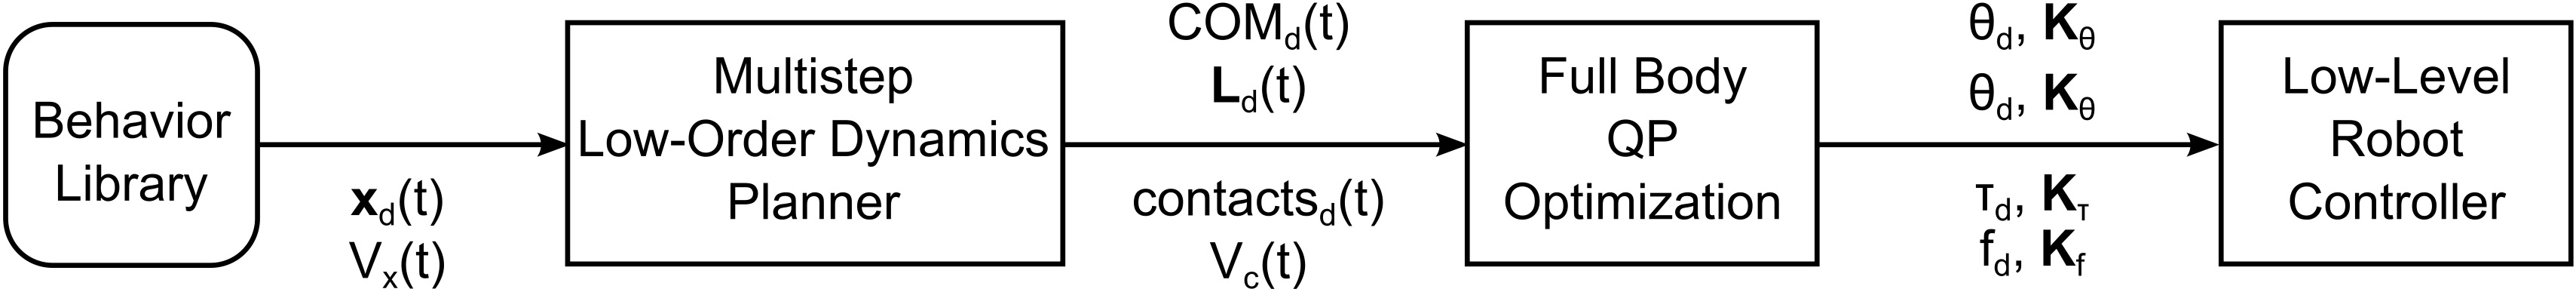
\includegraphics[width=0.75\textwidth]{Figures/cga1_modified}
\caption{Controller architecture based on hierarchical optimization.}
\label{f:cga1}
\end{figure}



\begin{figure}[t]
  \begin{center}
    {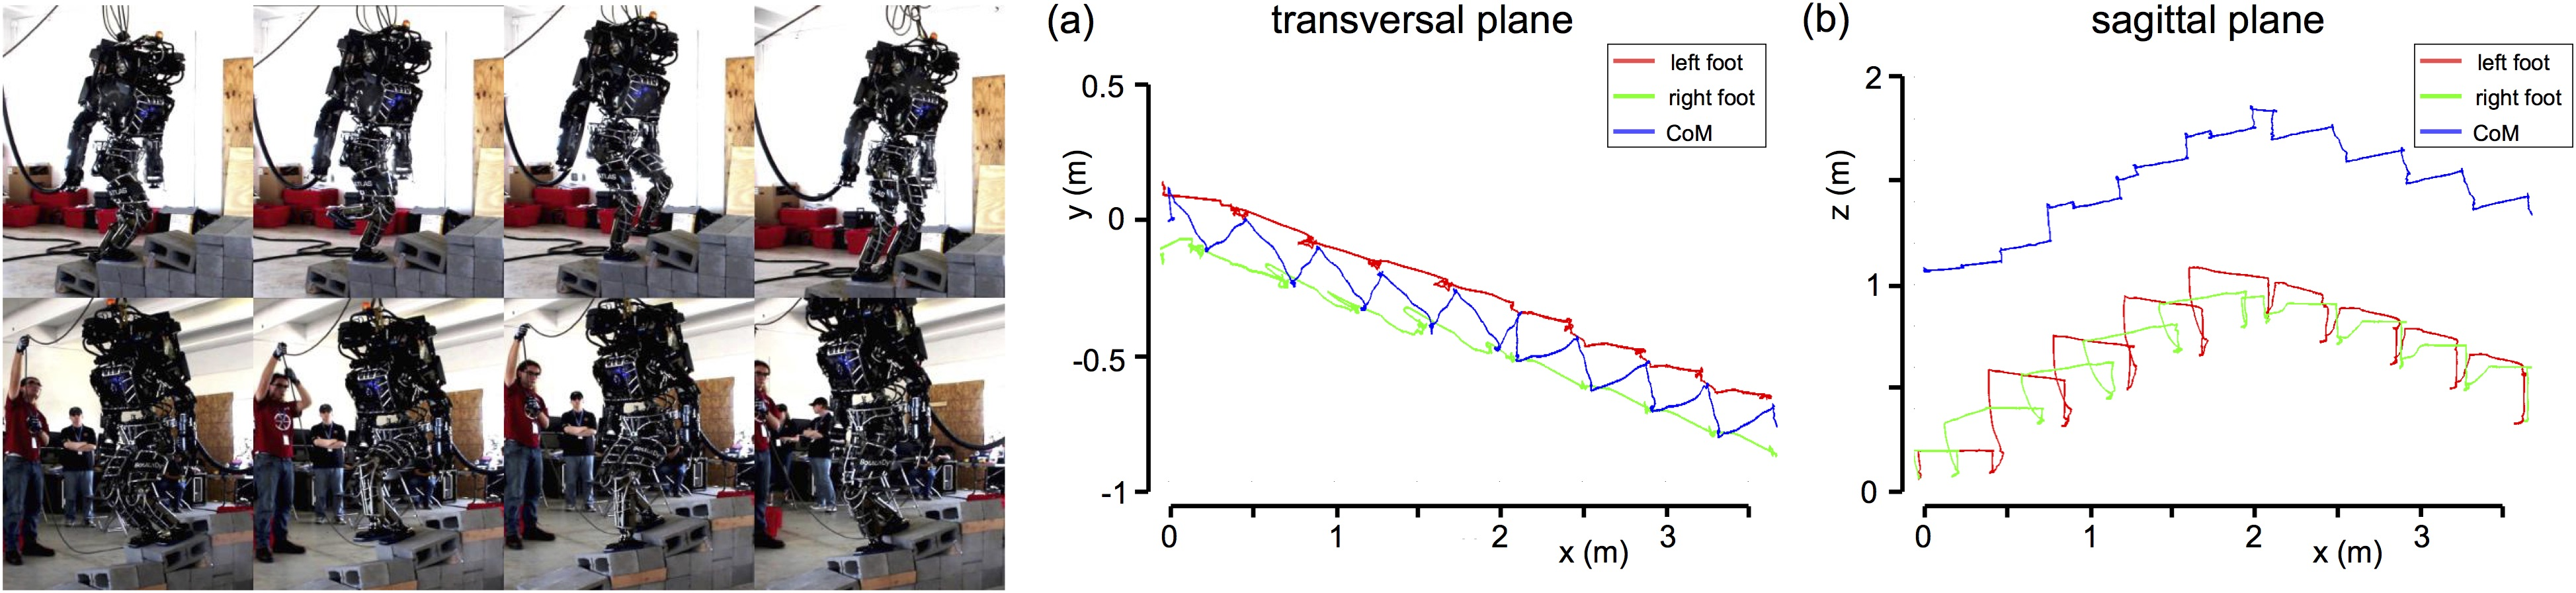
\includegraphics[height=3.8cm]{Figures/atlas_terrain}}
    \caption{ATLAS robot practicing for the terrain task of the DRC. Photo snapshots taken every 5 seconds. Measured trajectories in the transverse (a) and sagittal planes (b) of the left (red) and right foot (green) and the center of mass (CoM, blue) are shown. The robot walks in a straight line along $y=0$ in reality. Our state estimator at that time drifted significantly. This has been fixed by adding vision-based SLAM.
      }\label{fig:terrain_data} 
\label{fig:terrain_pic} 
  \end{center}
\end{figure}   


\begin{figure}[t]
  \begin{center}
    {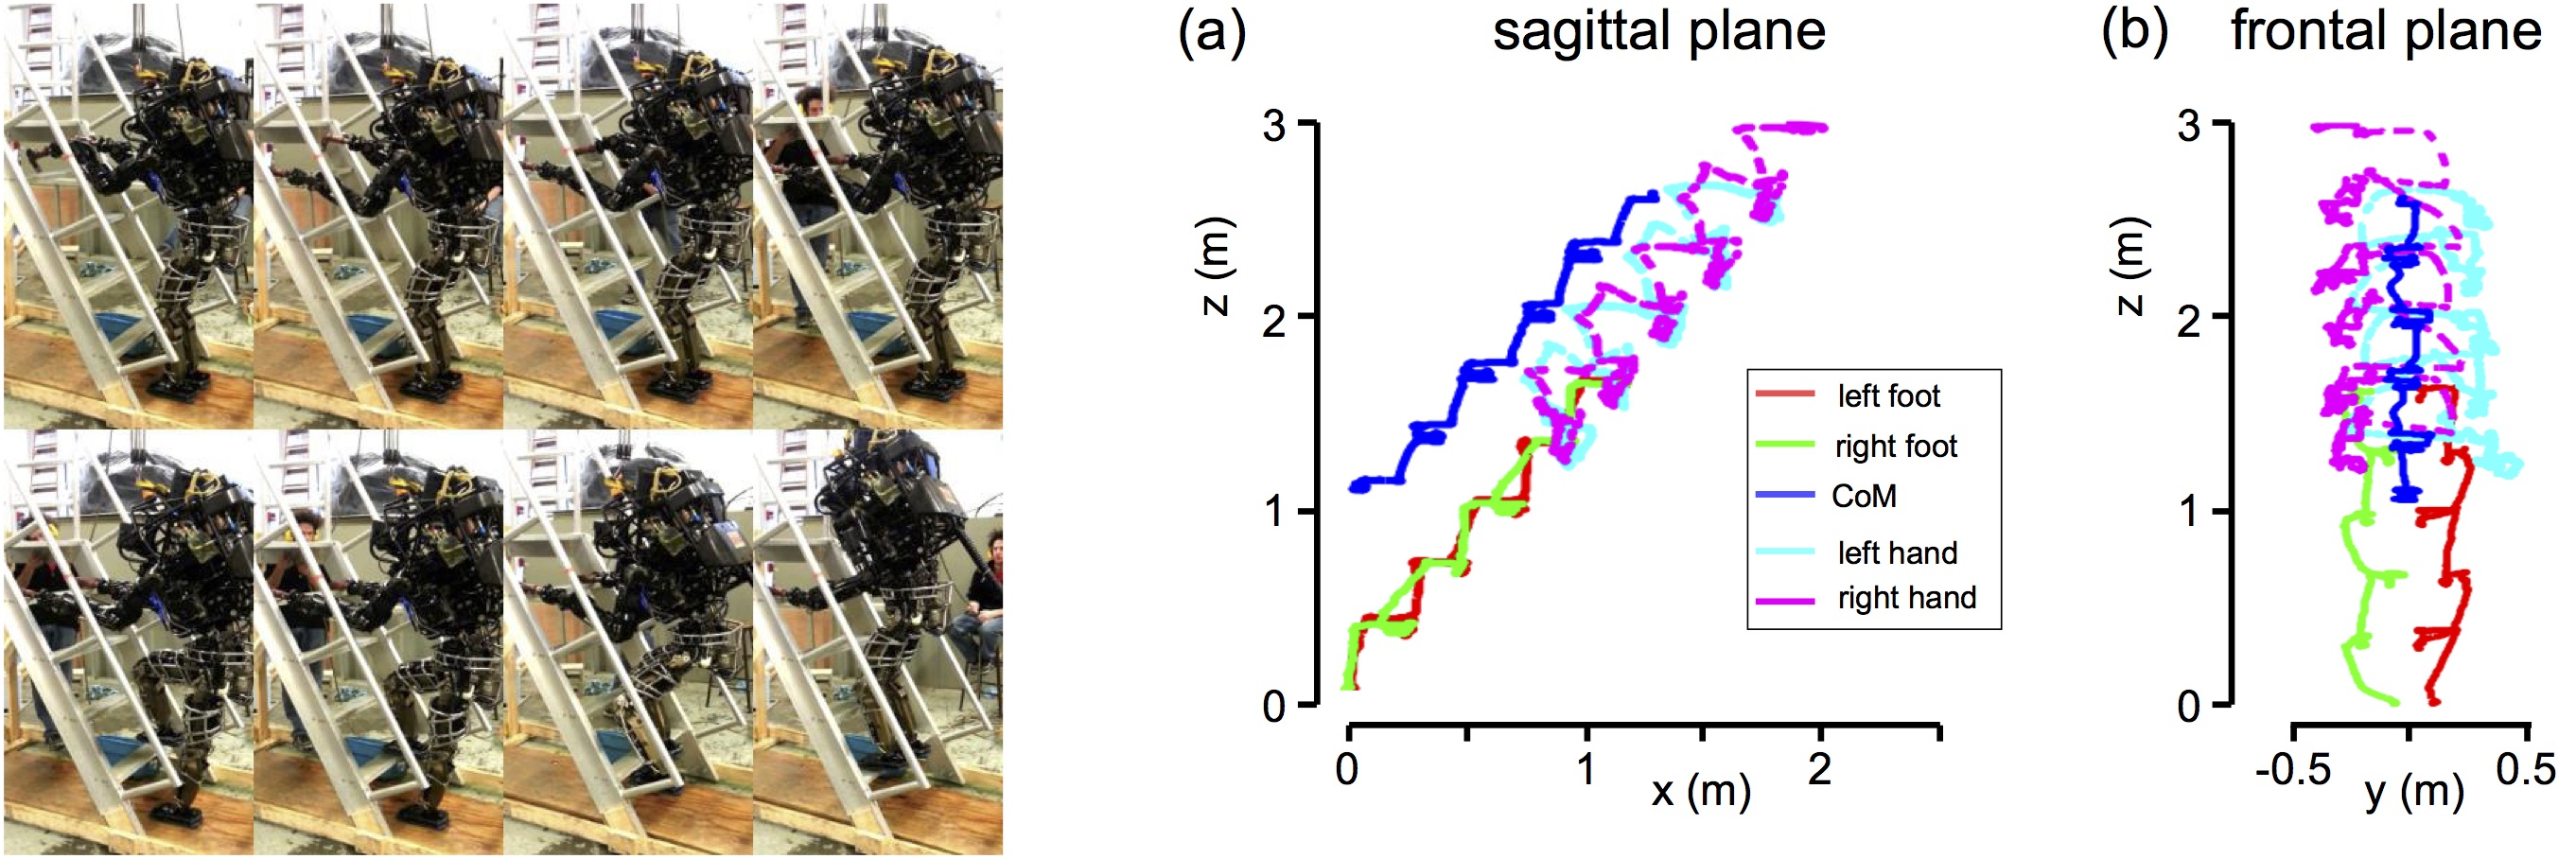
\includegraphics[height=4cm]{Figures/atlas_ladder}}
    \caption{
      ATLAS climbing the top half of the same 
      ladder as used in the DRC. Photo snapshots taken every 13 seconds. The
      top row shows repositioning of the hook hands, and the bottom row shows
      stepping up one tread.
      The two plots show ATLAS climbing the first five treads during
      the actual run at the DRC Trials. Axis definitions and color codes for foot and CoM trajectories are the same as in Fig.~\ref{fig:terrain_data}. Left and right hand positions are plotted with cyan and magenta dashed lines. 
      }\label{fig:ladder_data} 
\label{fig:ladder_pic} 
  \end{center}
\end{figure}    

In the controller architecture, the {\bf Behavior Library} (Fig.~\ref{f:cga1}) contains
learned behaviors and behaviors created from demonstration or
motion capture of humans or other robots, and also acts as a cache
for planning. The output of the library is used to prime, speed up,
and guide the real time optimization process, and can be motion
or force trajectories in joint or task coordinates ($\vx_d(t)$), as well as
possibly including value, heuristic cost, or utility functions ($V_x(t)$)
that can be used
to guide search and optimization. 
Libraries can be built in advance, or when task specification are known.
The rest of the controller can
also operate without information from the library if suitable information
is not available.

The {\bf Multistep Low-Order Dynamics Planner} uses
receding horizon control to continually optimize trajectories of
motion and force of a simplified model of the current task.
In walking, this is usually center of mass ($COM_d(t)$),
angular momentum ($\mL_d(t)$),
contact force ($\mbox{contacts}_d(t)$) trajectories,
and value, heuristic cost, or utility functions ($V_c(t)$)
specifying tradeoffs between these quantities.
We optimize with a time horizon of several seconds
using Differential Dynamic Programming~\cite{ddp}.

For walking, our planner is similar in spirit to Kajita's Preview Control for a Linear Inverted
Pendulum Model (LIPM)~\cite{kajita03}. We are also using a CoM
model, reason about Zero Moment Point (ZMP), and use future information 
to guide the current trajectory. However, our planner can be generalized to 
nonlinear models and adjust foot steps while optimizing the CoM 
trajectory. 
%We explicitly add the vertical height in our  CoM model to handle height variations on rough terrain. 
Like capture point methods~\cite{capture_pt}, we take the 
next few steps into consideration but
do not plan to come to rest at the end. Ogura et al.~\cite{wabian2} 
investigated generating human-like walking with heel-strike and toe-off by 
parameterizing the swing foot trajectory. In contrast, we use very simple rules to guide the low level controller to achieve the same behaviors.

The {\bf Full Body QP Optimization} uses quadratic programming (QP) with a
very short time horizon (1ms on SARCOS and 2ms on ATLAS) to optimize the 
desired full state of the robot ($\vtheta_d$, $\dot{\vtheta}_d$),
joint torques ($\vtau_d$), and contact forces ($\vf_d$).
Currently, we pre-specify gain matrices 
($\mK_{\theta}$, $\mK_{\dot{\theta}}$, $\mK_{\tau}$,
$\mK_{\mbox{f}}$)
for the robot controller, but plan to explore how to optimize gains
as well as trajectories.
This module enforces constraints
such as robot kinematics and dynamics 
and joint, velocity, torque, actuator, friction cone,
and center of pressure limits, and resolves redundancies.
The module performs inverse kinematics and dynamics to provide us with
compliant motions and dynamic behaviors, while compensating for the
effects of modeling errors.

For the QP, we use a formulation developed in our group 
\cite{Stephens-thesis,Whitman10,Whitman-thesis}. Unlike~\cite{mistry10,usc_id1} who 
use orthogonal decomposition to project the allowable motions into the null 
space of the constraint Jacobian, and minimize costs in the contact constraints and the commands, we directly 
optimize a quadratic cost in terms of state accelerations, torques and contact 
forces on the full robot model. This design choice allows us to trade off physical quantities of 
interest. We are also able to directly reason about inequality constraints 
such as center of pressure within the support polygon, friction, and torque 
limits. Although it becomes a bigger QP problem, we are still able to solve it 
in real time. Hutter el al.~\cite{eth_id} resolved redundancy in inverse 
dynamics using a kinematic task prioritization approach that ensures lower 
priority tasks always exist in the null space of higher priority ones. In 
contrast to their strictly hierarchical approach, we minimize a sum of 
weighted terms. 
We can directly specify the relative importance of the terms by adjusting 
the weights. 

%One popular approach to controlling humanoid robots is through inverse 
%kinematics with stiff joint position tracking. On the other hand, 
%inverse dynamics
%based approaches have gained increasing acceptance by providing compliant 
%motions and robustness to external perturbations. 
%However, the performance of inverse dynamics methods 
%is heavily dependent on high quality dynamic models, which are often very 
%difficult to produce for a physical robot. In contrast, inverse
%kinematics based approaches 
%only require kinematic models, which are much easier to generate in practice. 
%This was one reason we supplemented our original two part implementation with 
%an inverse kinematics controller for the physical robot.



The {\bf Low-Level Robot Controller} is a blend of our work and controllers
provided by the robot manufacturers. For SARCOS
and ATLAS, hydraulic valve commands for each
joint $i$ are generated by high rate servo controllers provided
by the manufacturers,
\begin{equation}
v_i = k_{\theta,i} ( \theta_i - \theta_{d,i} )
+ k_{\dot{\theta},i} ( \dot{\theta}_i - \dot{\theta}_{d,i} )
+ k_{\tau,i} ( \tau_i - \tau_{d,i} )
+ v_{\ff,i}
\end{equation}
where $v_i$ is the valve command,
$\theta_i$ is the joint angle,
$\dot{\theta}_i$ is the joint angular velocity,
$\tau_i$ is the joint torque,
and $v_{\ff,i}$ is a feedforward valve command.
Subscripts $d$ indicate desired values, and
quantities denoted with $k$ are scalar gains.
This joint level servo runs at 5kHz on SARCOS and at
1kHz on ATLAS.

We augment this independent joint control by coupling joints
and providing force control based on force/torque sensors in the wrists,
ankles, and skin of the robot,
\begin{equation}
\vv = \mK_{\theta} ( \vtheta - \vtheta_{d} )
+ \mK_{\dot{\theta}} ( \dot{\vtheta} - \dot{\vtheta}_{d} )
+ \mK_{\tau} ( \vtau - \vtau_{d} )
+ \mK_{\mbox{f}} ( \vf - \vf_{d} ) 
+ \vv_{\ff}
\end{equation}
where $\vv$, $\vtheta$, $\dot{\vtheta}$, $\vtau$, and $\vv_{\ff}$
are the corresponding vector quantities, and the $\mK$ are matrix gains
coupling all joints. $\vf$ are sensed contact forces.
The coupled controller runs at 1kHz on SARCOS and 500Hz on ATLAS.

Figure~\ref{f:cga1} does not include our state estimator, which provides
appropriate state information to all other modules. The details of this work on state estimation are
described in~\cite{xinji_com_est,Xinjilefu-thesis}.

\section{Operator-Exoskeleton Force Control using position controlled actuation}

We will now consider position controlled actuators.
At this point our dynamics formulation is no longer appropriate, since we
are assuming the actuators are now position rather than torque sources.

\subsection{Get out of the way control with position sources}

The exoskeleton moves as to create as little force as possible between the
operator and the exoskeleton. The actuators in this case may be position sources or
force sources with high servo gains,
but ultimately operator-exoskeleton forces are mapped
to exoskeleton velocities or angular velocities.

\begin{equation}
\dot{\vq}_d = \mJ^{-1} (\mK_1 \vf)
\label{eq:gootwcps}
\end{equation}
where $\dot{\vq}_d$ are the commanded exoskeleton joint velocities,
$\mJ$ is an appropriate Jacobian matrix, $\mK_1$ is a gain matrix,
and $\vf$ is the force vector to be controlled~\cite{IEEE06990981}.

Inverting a Jacobian matrix is problematic when the matrix is
nearly singular.
Using a fixed or gain scheduled gain matrix may make more sense.
\begin{equation}
\dot{\vq}_d = \mK_3 \vf
\end{equation}
Simplifying equation~\ref{eq:gootwcps}
by assuming the forces to be controlled
are directly applied to the exoskeleton joints, and thus the Jacobian matrix
is the identity matrix, gives us a similar equation:
\begin{equation}
\dot{\vq}_d = \mK_1 \vtau_{\ox}
\end{equation}
and we avoid inverting a Jacobian and problems with singularities.

\subsection{Operator force feedback with position sources}

We introduce a desired force to allow for more complex force control.
\begin{equation}
\dot{\vq}_d = \mJ^{-1} (\mK_1 (\vf - \vf_d))
\end{equation}

The exoskeleton could move as to provide a scaled version of exoskeleton-world
contact forces, or some other (usually simple) mapping. 
\begin{equation}
\vf_d = \alpha \mJ_{ow} \vf_w
\end{equation}

\section{State Estimation}

We have not seen a lot of discussion of state estimation of exoskeletons in
the literature.
We will discuss our approach to state estimation on humanoid robots here.
State estimation to deal with sensor noise,
disturbance estimation, and incomplete or
redundant sensing is a separate process and is as independent as possible
from the control method~\cite{certainty-eq,separation-prin}.
This makes evaluating different control methods much easier.
Disturbance observers for disturbances such as
moving support surfaces, contact or wind forces, and model errors
are also implemented.

For humanoid robot state estimation (for proposed exoskeleton state estimation)
we use extended Kalman Filtering (EKF) to perform state estimation.
Currently, using the full body dynamics 
(equations~\ref{eq:xdynamics2} or \ref{eq:oxdynamics2})
and any additional constraint equations for ground contacts (feet on the ground):
\begin{equation}
\mJ_w \ddot{\vq} + \dot{\mJ}_w \dot{\vq} = 0
\end{equation}
is too expensive to produce both a forward prediction and a linearized model
about the current state in the desired 1ms time step.
Therefore we approximate the dynamics by separating the center of mass dynamics
from the joint dynamics and use two separate extended Kalman filters:
a filter for the center of mass dynamics, and a filter for the joint dynamics.
We use an orthogonal (QR) decomposition to project motion into the orthogonal
complement of the contact Jacobian where the ``external'' dynamics (the dynamics
of the center of mass) are separate from the ``internal'' dynamics (the motion
of the joints).

Joint velocities are estimated using actuator position sensors, actuator load
sensors, actuator commands, a single high
quality IMU at the pelvis, and multiple low quality (but cheap) MEMs IMUs
spread throughout the robot or exoskeleton. We also take into account feet and hand
contact forces, which
are measured. We use the full internal dynamics as the process model,
assuming the root dynamics are known. See Chapter 3 of~\cite{Xinjelefu-thesis}.
The internal dynamics are linearized and covariances updated
by a separate process at a 100Hz rate.
The joint positions are predicted by integrating the estimated velocities.

For higher level (overall) state estimation,
we developed a center of mass location and velocity estimator~\cite{}.
The center of mass filter is modeled as a multiple model EKF with contact switching
to handle changes in support: single support, double support, and off the ground.
We use the robot or exoskeleton
joint sensing (kinematics) to create a virtual sensor that measures
center of mass position and velocity relative to a stance foot.
We use Linear
Inverted Pendulum Model (LIPM) dynamics with an offset to predict
the center of mass motion. This offset can be interpreted
as a modelling error on the center of mass position, or an
external force exerted on the center of mass of the robot/exoskeleton,
or a combination of both. The center of mass estimator was
implemented on our Atlas humanoid robot. 
This estimator is especially helpful when compensating
for unplanned slow changing external forces applied at
unknown locations on the robot or exoskeleton, which is quite likely when
operating in tight spaces. It also handles relatively small
dynamic forces well when walking, e.g. dragging a tether
or pushing through a spring loaded door. Thanks to
the estimator, very little tuning is done for our mass model.
During the DARPA
Robotics Challenge Finals
where no safety belay was
allowed, our fall early warning system based on this estimator
successfully saved our robot from
falling on two occasions, and made us the only competitive team
without a fall or need for a human rescue among all teams.

{\bf Safety Code: Fall Prediction:}
The most significant contribution of the external force estimator is that it
can detect when a large external force is being applied that might
push the robot or exoskeleton over.
We compute a ``corrected capture point'' (CCP)~\cite{capture},
which is an offset to the current capture point.
The offset 
takes into account the estimated external force, represented as an offset
to the center of mass.
The corrected capture point getting close to the boundary of the polygon of
support warns the controller that the robot or exoskeleton might fall if the external
force is maintained.
We can also compute the corrected capture point assuming that the
external force follows a known time course plus an estimated constant offset,
or steadily increases or decreases for a fixed time interval
based on an estimated derivative.
We assume the external force is due to the robot's or exoskeleton's
movements, and not
due to external disturbances such as wind, a moving support platform
or external agents pushing on the robot.
The current
behavior is stopped and the robot or exoskeleton can safely be ``frozen'' in place.

A derivation of the corrected capture point starts with LIPM dynamics
augmented with a true center of mass offset and a true external force:
\begin{equation}
\ddot{c} = (c + c_{offset} + f_{ext}*z/mg - cop)*g/z
= (c + \Delta - cop)*g/z
\end{equation}
where $c$ is the location of the center of mass projected on the ground
plane,
$cop$ is the center of pressure
location in that ground plane, and $\Delta$ is the sum of the true center of mass
offset from the modeled center of mass and any external horizontal force.
Our extended Kalman filter estimates $\hat{c}$, $\hat{\dot{c}}$, and
$\hat{\Delta}$,
taking into account the
current center of mass height $z$. We assume a constant center of mass height
in estimating the corrected capture point based on the estimated capture point
as described in~\cite{capture}:
\begin{equation}
\widehat{CCP} = \widehat{CP} + \hat{\Delta} 
= \hat{c} + \hat{\dot{c}}\hat{z}/g + \hat{\Delta}
\end{equation}

For dynamic walking, the corrected capture point goes beyond the
current single foot support polygon during swing phase and is captured by
the touchdown foot. One way to predict a fall is to use the
swing foot time to touchdown and predict if the current
capture point is within the support polygon of possible or desired
footholds. This approach is complicated because it depends
on the controller. Our simpler solution is to use a heuristic
that detects a fall only if the corrected capture point
is outside of the current support
polygon for a continuous period of time. The time threshold was set to
0.6 seconds after extensive testing. As soon as a fall is
predicted, there are several things the humanoid or exoskeleton can do, such
as using angular momentum to maintain balance, or changing the
current or future foot placements.
We have implemented a simple
step recovery controller that works in single support where
the robot or exoskeleton corrects the next foot placement and timing
using a simple heuristic to avoid self collision.
We would only step left if the robot or exoskeleton is falling left, and similarly
for right steps. We avoid crossing the legs in using foot placement
to balance laterally.

\begin{figure}[t]
  \centering
  \hbox{}
      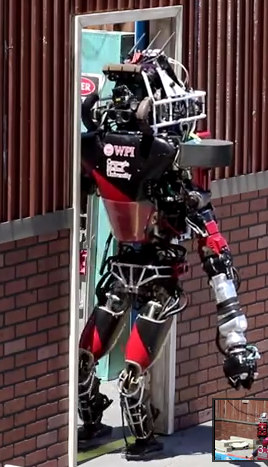
\includegraphics[height=5cm]{figs/door1-5.png}
%      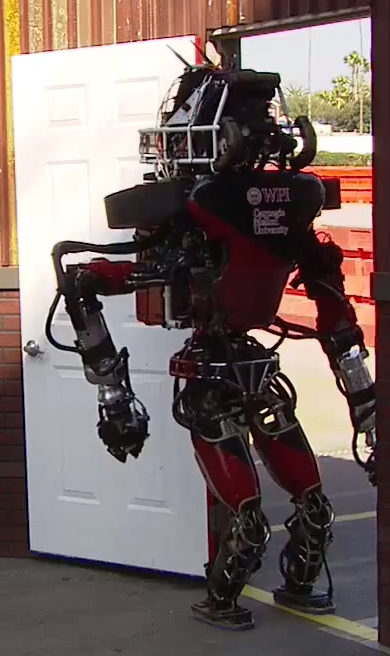
\includegraphics[height=5cm]{figs/door2-1c.png}
      \hbox{}
      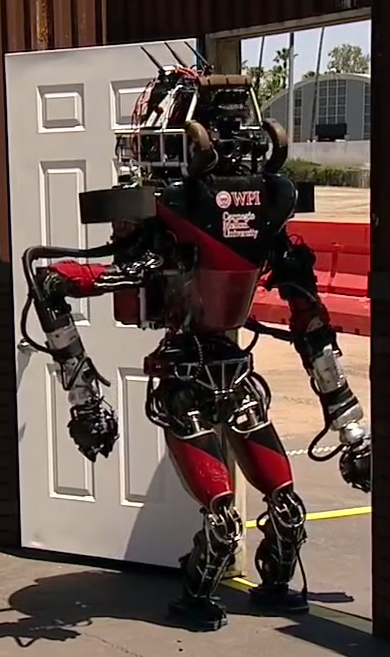
\includegraphics[height=5cm]{figs/door1-3.png}
      \hbox{}
      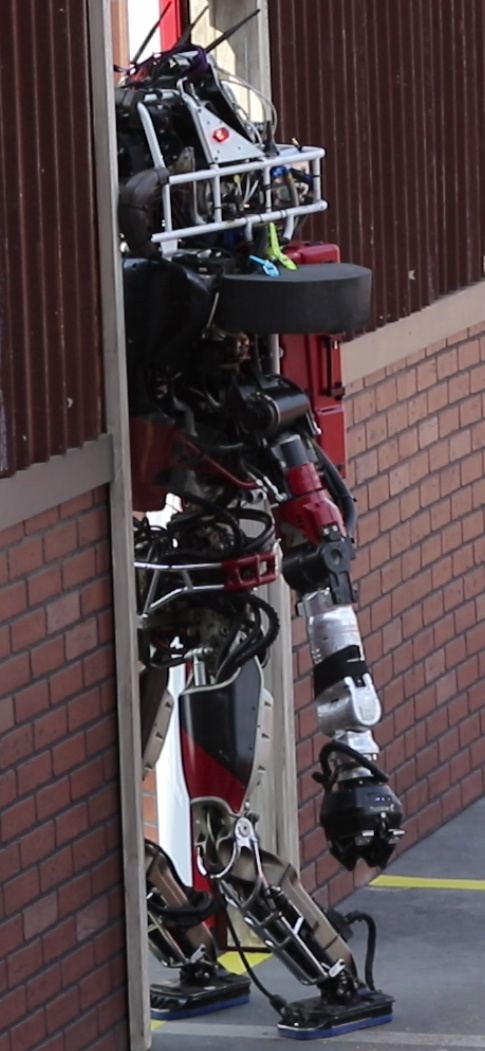
\includegraphics[height=5cm]{figs/door-stuckc2.png}
      \hbox{}
      \caption{Successful sidestepping through the door (left, middle)
        and the failure in the DRC rehearsal (right) in which the protective
        cage (black padding) for the head is against the white door frame.}
      \label{figDoor}
\end{figure}

\begin{figure}[t]
      \centering
      % 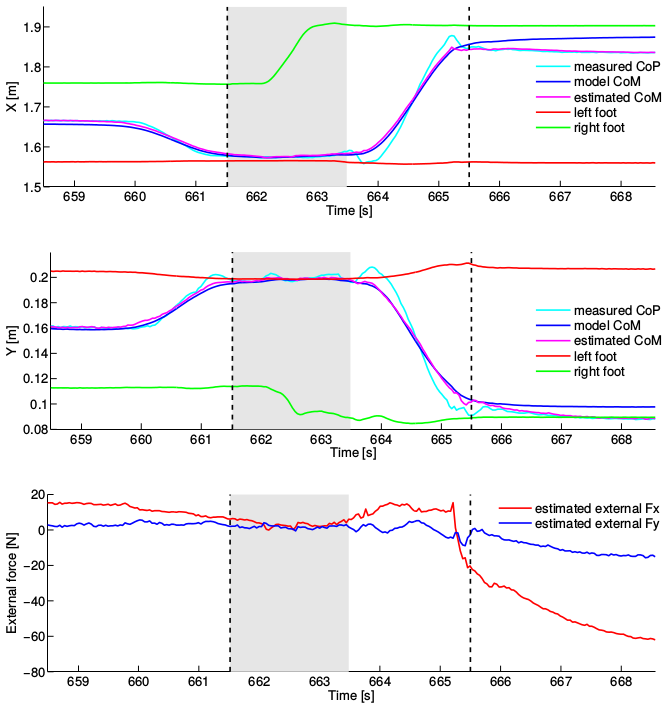
\includegraphics[width=0.48\textwidth]{figs/door-traces.png}
\subfigure
{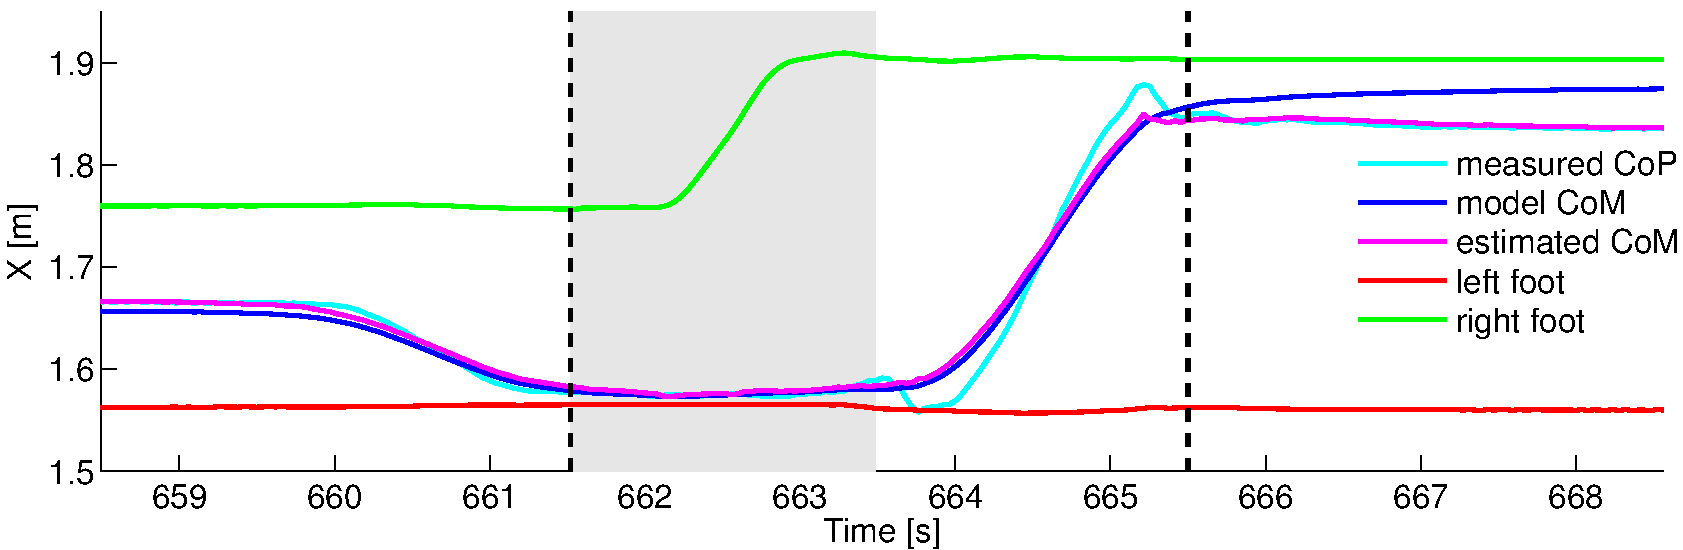
\includegraphics[width=0.48\textwidth]{figs/cop_x1.pdf} \label{subfig:ext_cop_x}}
%\subfigure
%{\includegraphics[width=0.48\textwidth]{figs/cop_y.pdf} \label{subfig:ext_cop_y}}
\subfigure
{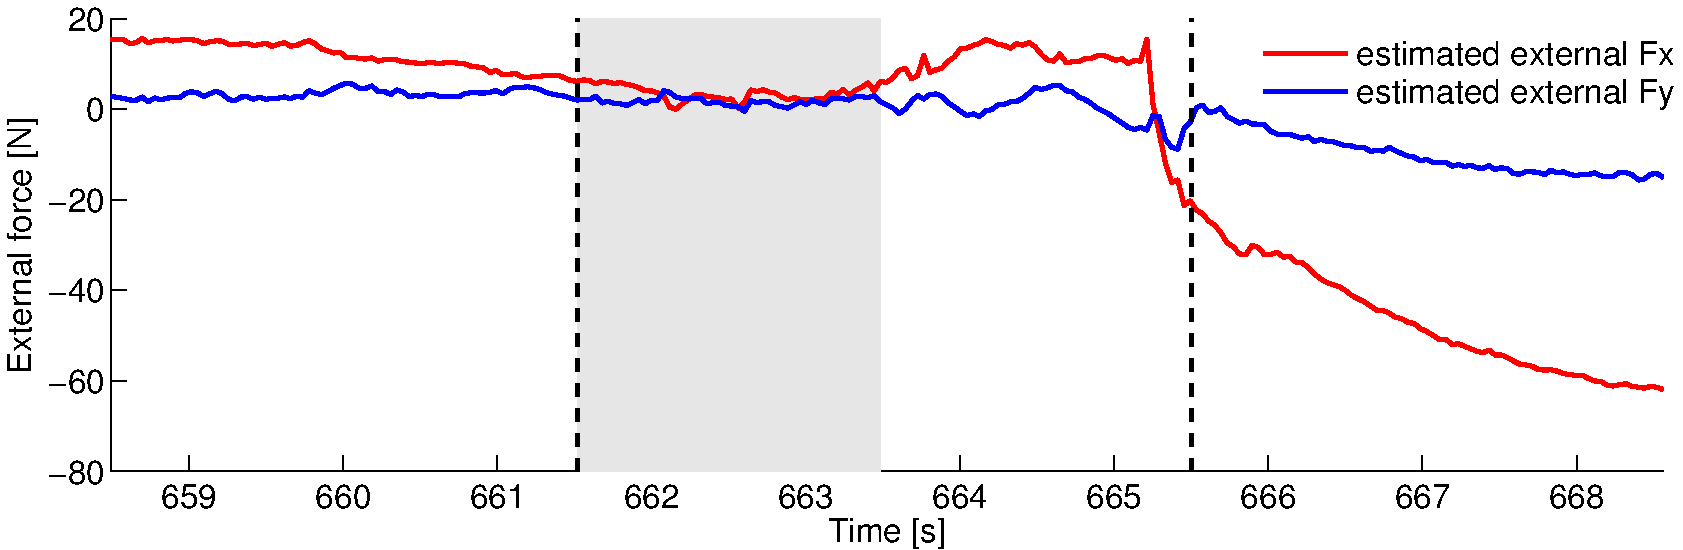
\includegraphics[width=0.48\textwidth]{figs/ext_f1.pdf} \label{subfig:ext_f}}
\caption{
Atlas was caught on the door frame when sidestepping through it during
the DRC rehearsal.
The walking controller delayed liftoff and remained in double
support when the external force estimator detected a large change
in the estimated external force in the robot's sideways
direction ($F_x$, through the door).
The single support phase is shown by the shaded area, and the black dashed
lines indicates the planned liftoff time.
The estimated CoM is the sum of the model CoM and the estimated CoM offset.
}
\label{figDoorError}
\end{figure}

{\bf Results of Safety Code: Robot caught on door frame:}
In the DRC rehearsal, the robot was caught on
the door frame when sidestepping though (Figure~\ref{figDoor}).
The walking
controller detected an anomaly in the estimated external force in the
sideways direction ($F_x$),
delayed liftoff and remained in double support, and stopped the
current behavior
to allow for manual recovery (Figure~\ref{figDoorError}).

{\bf Results of Safety Code: Manipulation Error:}
For the manipulation controller, the robot is always assumed
to be in double support, and the support polygon
is computed by finding the convex hull of the foot corner
points (light green in Figure~\ref{figDrillCOP}),
computed using forward kinematics.
To prevent the robot from falling during
manipulation, we require the corrected capture point to be within a
subset of the support polygon called the safe region, 
(dark green in Figure~\ref{figDrillCOP}),
When the corrected capture point escapes the safe region,
a freeze signal is sent to the manipulation controller, and it
clears all currently executing joint trajectories and freezes the robot
at the current pose, with the balance controller still running.

During our second
run in the Finals, our right electric forearm mechanically failed
when the cutting motion was initiated for the drill task. The
uncontrolled forearm wedged the drill into the wall and
pushed the robot backwards.
The controller stopped the behavior (a freeze),
and saved the robot from falling (Figure~\ref{figDrillCOP}).
The operator was then able to
recover from an otherwise catastrophic scenario.

The time plot in Figure~\ref{figDrillCOP} shows candidate fall predictors
during this event. We can eliminate some candidate fall predictors
easily. The center of mass (CoM) (and a ``corrected'' CoM (not shown))
usually provide a fall warning too late, because the CoM velocity is not
included. The capture point (CP) does not include information about
external forces. The center of pressure (CoP) is 
noisy and gives too many false alarms. It can warn of 
foot tipping, but it is less reliable about warning about robot falling,
which is not the same thing as foot tipping in a force controlled robot
or if there are non-foot contacts and external
forces. In this plot, we see that the CoP moves away from the safe region
during recovery, predicting that the robot is falling again, while the
corrected capture point (CCP) moves towards the interior of the safe region.

\begin{figure}[t]
      \centering
      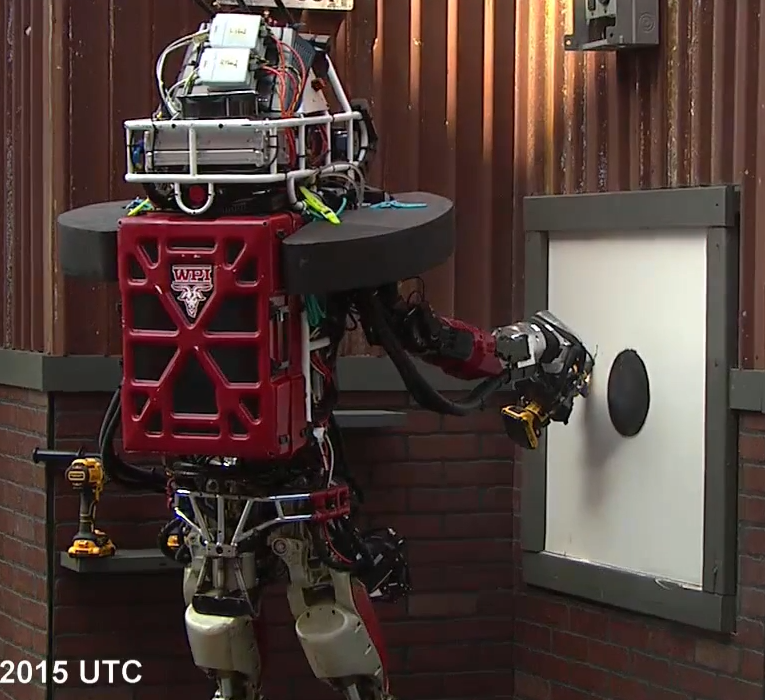
\includegraphics[height=30mm]{figs/near-fall2c.png}
      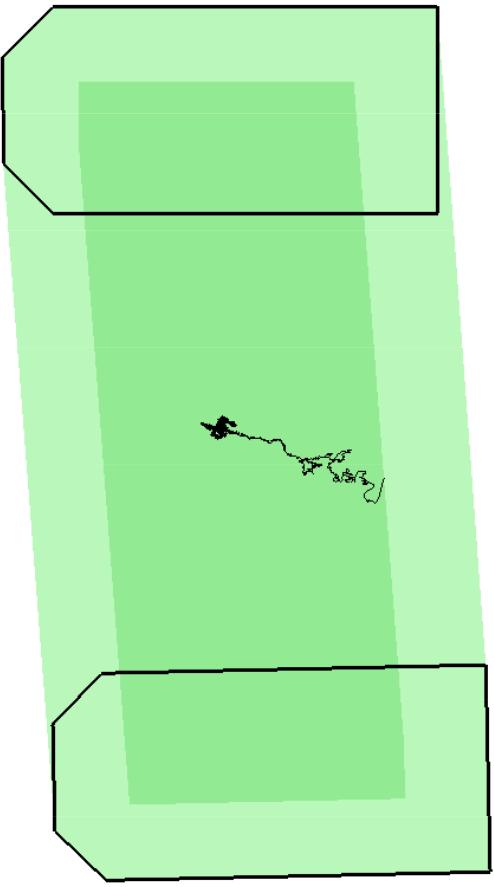
\includegraphics[height=30mm]{figs/drill-cop1.png}
      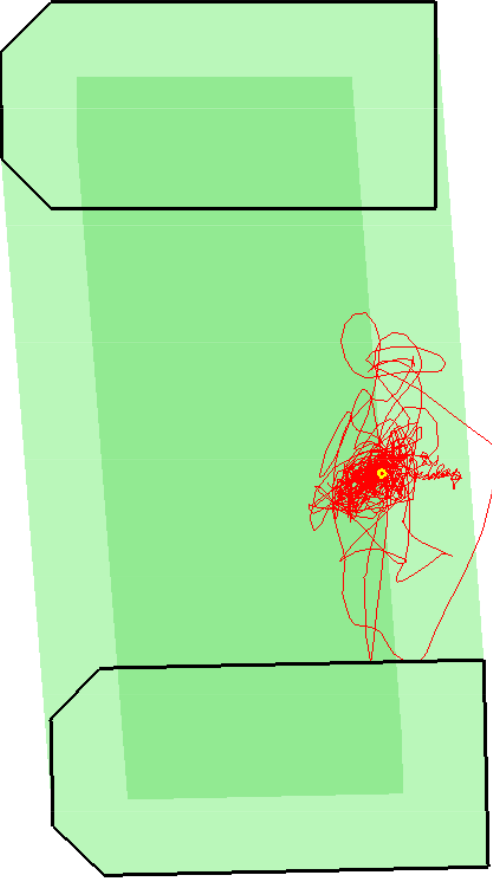
\includegraphics[height=30mm]{figs/drill-cop2.png}
      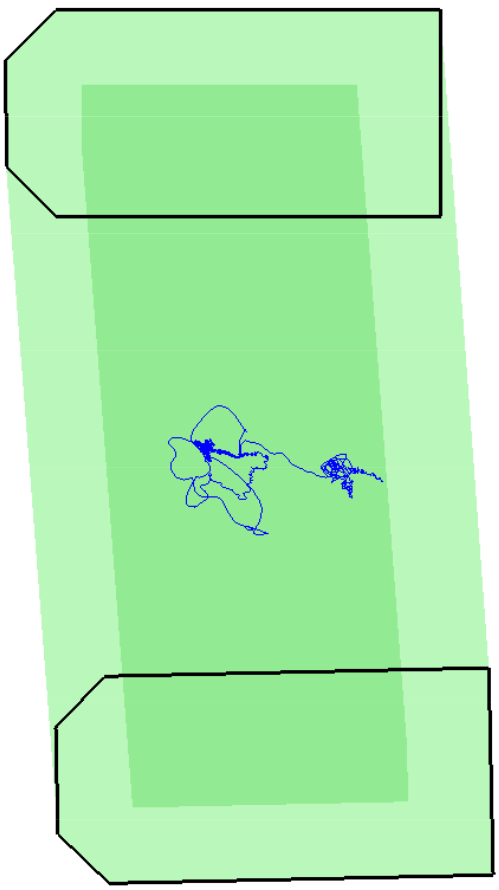
\includegraphics[height=30mm]{figs/drill-cop3.png}\\
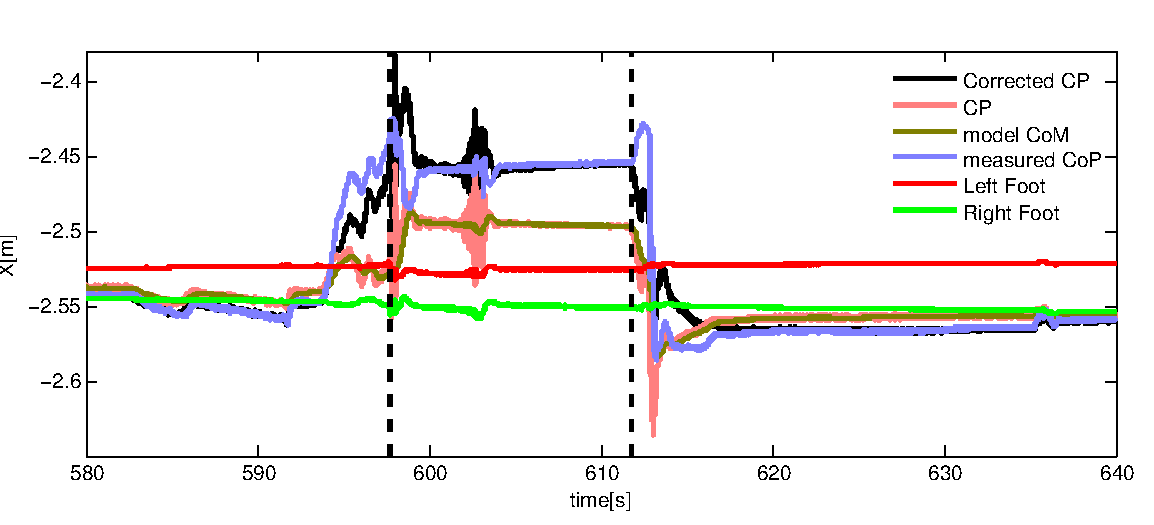
\includegraphics[width=0.48\textwidth]{figs/cp_time_xes.pdf}
      \caption{Top Left: Robot posture after 
error detection.
Top Right: Black trace: The corrected capture point (CCP)
up to the error detection,
Red trace: The CCP during the ``frozen'' period, and Blue trace: The CCP moves
back to the center of the polygon of support during manual recovery.
Bottom: Plots of candidate fall predictors in the fore/aft direction
during this event. The black vertical dashed lines mark the freeze time and
the start of manual recovery.}
      \label{figDrillCOP}
\end{figure}

Unscented and particle filters could be used instead of extended
Kalman filtering. It may well be the case that unscented filtering
outperforms extended Kalman filtering.

\subsection{Current state estimation approaches in exoskeletons}

We see that Sensitivity Amplification Control uses acceleration as an input.
Estimating acceleration using double differentiation with low pass filtering
currently works well on real exoskeletons.
However, impacts, shock waves, and the fact that neither
the operator's body parts or the exoskeletons parts are rigid bodies and the
joints are not well defined suggest this approach can be improved with actual
acceleration measurements.
It is now possible to distribute MEMs IMUs throughout the exoskeleton to
improve both velocity and 
acceleration estimation~\cite{Xinjilefu-thesis}, which should improve
Sensitivity Amplification Control.

Disturbance observers~\cite{IEEE06197032}.

\section{Robustness to parametric modeling error and unmodeled dynamics}

We need to be robust to parameter modeling errors such as the wrong mass,
center of mass location, joint location,
or moment of inertia for an exoskeleton part, variations in the operator
parameters, and variations in attachments to the exoskeleton and payload.
Examples of unmodeled dynamics (non-parametric modeling error) include:
backlash, joint play, structural deformation, flexible wires and hoses,
actuator dynamics, processing delay,
elastic operator tissue and straps, and 
loose or slack operator tissue and straps.

There are two questions to focus on:

\subsection{How robust are these control schemes to parametric and non-parametric
modeling error?}

This question needs to be addressed using simulation, and is deferred to a 
possible future white paper [robust.pdf].

\subsection{How can we make control more robust?}

One way to understand control systems is to separate 1) what happens when there
are no errors and feedback control is not active, and 2) what happens in response
to errors (feedback control). 
What happens when there are no errors in model-based control is 
feedforward control, which does not have stability issues (except for some ignorable
technical issues). If your model is good, you get good performance. If your
model is bad, you get larger errors and have to rely on feedback control.
You may crash the exoskeleton, or fall down, but you will not oscillate
(except in some contrived examples) and errors do not grow exponentially in
response to feedforward control errors (except for unstable and chaotic systems).
So feedforward control is technically robust,  
and we don't have to worry about it going wildly out of control.
We do have to worry about performance.
We have
to worry about how to get good models, and what to do about stuff that varies:
contacts, operator body, operator behavior, payloads, attachments, etc.

On the other hand, feedback control can lead to steady state or growing
oscillation, which we colloquially refer to as being unstable or instability.
Since walking and running are also oscillations which we refer to as stable
behaviors, the technical meaning of the word ``stable'' is more complex than
just ``it keeps moving'' or ``it doesn't do what the operator wants''.
In any event, we don't want oscillations.

The best way to avoid oscillations is to manually design a conservative 
independent joint feedback controller.
This way it can be tested independently of any
feedforward control.
Unfortunately, inverse dynamics and online optimization-based control mix
feedforward and feedback control so we cannot use the recommended, well established,
and safe approach of manual conservative independent joint feedback control design. 

What to do about this to achieve robust online optimalization-based control is
currently a research issue. In actual implementations, skilled engineers manually
tune optimization weights and the various constraints that are active to
make this type of control work reliably. The fact that this has been done on many actual
humanoid robots in many situations is comforting. The fact that none of these
implementations have moved with the speed and agility of a top percentile
human athlete is disconcerting.

We can ``verify'' designs using simulation, but making accurate simulations of
the effects of contact and unmodeled dynamics is also a current research issue.
There is no getting around the fact that our operators will be like the test
pilots of early planes. The exoskeletons may crash, flail wildly, or oscillate.
We need to plan for operator safety from day 1 of operation, not try to retrofit
it later.

If the robustness of online optimization is not adequate, an alternative is
combining feedforward and feedback control into one function and using gradient
descent in simulation to improve the control robustness.
One technique to do this is multiple-model design~\cite{acc12}.

Note that adaptive or learning
control does not promise to improve the kind of robustness exoskeletons need. 
These approaches promise
to improve performance, and try to track (slow) changes in the operator, exoskeleton,
or contacts to maintain performance. If something changes quickly, we need robust
control design.

\section{Specific Proposed and Implemented Exoskeleton Control Schemes}

\subsection{Sensitivity Amplification Control}

Sensitivity Amplification Control (SAC) used to control BLEEX
is a dynamic cancellation technique (a.k.a.
inverse dynamics, computed torque, or feedback linearization) that also tries
to modify the apparent inertia of the exoskeleton (equation~\ref{eq:change-inertia1})
using acceleration feedback. It is not clearly stated but it appears that the
acceleration is the result of double differentiating position, as there do not
appear to be velocity sensors on BLEEX. Low pass filtering is applied to reduce
the high frequency noise amplified by the double differentiation process.

\subsection{Integral admittance control}

{\it [Exoskeletons] have the implicit property
of causing a virtual modification of the dynamic response of
the human limb. We use this property of the exoskeletons
action to formulate a unified control design framework called
Integral Admittance [torque to angle] Shaping, which designs exoskeleton con-
trollers capable of producing the desired dynamic response
for the assisted limb. In this framework, a virtual increase
in the admittance of the limb is produced by coupling it
to an exoskeleton that exhibits active behavior. Specifically,
our framework shapes the magnitude profile of the integral
admittance (i.e. torque-to-angle relationship) of the coupled
human-exoskeleton system, such that the desired assistance is
achieved. This framework also ensures that the coupled stability
and passivity are guaranteed.}~\cite{Nagarajan_etal_2015}

{\it ... the impedance of the coupled human-exoskeleton
system needs to be reduced below that of the unassisted
human limb. This implies that the exoskeleton needs to
cancel its own impedance first and then compensate for
at least a part of the human limb’s impedance. Therefore,
the desired exoskeleton behavior must be that of a negative
impedance ... Consequently,
the feedback gains will all be
positive. In other words, the exoskeleton controller uses
positive feedback, and hence the exoskeleton exhibits active
behavior, which is capable of performing net positive work
on the limb. ...
However, positive feedback naturally raises the question of
stability, and so we now explain how coupled stability can be
achieved. Although the exoskeleton exhibits active behavior,
which can be potentially destabilizing, the controller can be
designed such that the coupled human-exoskeleton system
is stable and passive. ... 
}~\cite{Nagarajan_etal_2015}

{\it
... Inertia compensation is more complex ...
It can be shown that using only positive acceleration
feedback ..., the gain margin of the coupled system
reduces to the moment of inertia of the exoskeleton, which
implies that the exoskeleton controller ... can at the most
compensate for the exoskeleton’s own moment of inertia
before going unstable. This implies that the moment of
inertia of the coupled human-exoskeleton system cannot be
reduced below that of the unassisted human limb, without
compromising coupled stability. However, using low-pass
filtered acceleration feedback, it can be shown that inertia 
reduction can be achieved. ...
This work uses filtered acceleration
feedback with a second-order low-pass Butterworth filter. ...
}~\cite{Nagarajan_etal_2015}

This is a form of frequency domain virtual model control.

\begin{verbatim}
Kalman filter:
P. Canet, “Kalman filter estimation of angular velocity and accelera-
tion: On-line implementation,” McGill University, Montr ́eal, Canada,
Tech. Rep. TR-CIM-94-15, Nov. 1994.
\end{verbatim}

\subsection{Dual Control Approach}

This approach implements a passive leg swing in addition to Sensitivity 
Amplification Control for the stance leg.

{\it The robot utilized the dual-mode control scheme, which is
comprised of the active control for the stance phase and the
passive control (using bypass valves) for the swing phase, to achieve high walking
speed in the swing phase while supporting heavy loads in
the stance phase. To reduce the sudden change of the torque
command at the transition from the swing phase to the stance
phase, a smoothing method is adopted. We also implemented
a pre-transition method to take a foot off quickly for fast
walking by predicting the change from the swing to the stance
in advance.}~\cite{IEEE07222598}

%Bypass valves implement what Sarcos calls ``dangle''.

Stance: virtual joint torque control method Kazerooni et al.(2005)
When contact location between the wearer and the
exoskeleton is not fixed and difficult to estimate, this method
has been shown to be an effective method to generate the
locomotion for an exoskeleton robot.[3],[4],[21]
\begin{verbatim}
H. Kazerooni , Z. Racine , L. Huang and R. Steger ”On the control of
the Berkeley lower extremity exoskeleton (BLEEX),” Proc. IEEE Int.
Conf. Robot. Autom., pp. 4364-4371, 2005.
Racine Jean-Louis Charles ”Control of a Lower Extrmity Exoskeleton
for Human Performance Amplification,” University of California,2003.
582
Xiuxia Yang, Hongchao Zhao, Yi Zhang, Xiaowei Liu ”Carrying
Lower Extreme Exoskeleton Rapid Terminal Sliding-Mode Robust
Control,” Journal of computers, vol.9, No.1,202-208. 2014.
\end{verbatim}

To reduce
sudden changes(command jump) at the phase transitions, a
smoothing method [5],[19] is introduced and a pre-transition
method is used to solve the swing delay due to the internal
pressure(approx 5 bar).
\begin{verbatim}
H. Kazerooni , Ryan Steger, Lihua Huang ”Hybrid Control of the
Berkeley Lower Extremity Exoskeleton (BLEEX),” Int. Journal of
Robotics Research, pp. 561-573, 2006.
oonbum Bae, Kyoungchul Kong, Masayoshi Tomizuka ”Gait Phase-
Based Control for a Rotary Series Elastic Actuator Assisting the knee
\end{verbatim}

Transition Control

1) Smoothing Method: During transitions of the gait
phase, discontinuity of the control command torque are
occurred by the different condition for the fixed coordinate
which is on the backpack at the swing phase or the foot at
the stance phase. In this paper, to reduce this sudden change
due to gait phase changes, a smoothing method is proposed
as shown in Fig. 7. An exponential function is considered
as the weighting function for smoothing as shown in (6).
In this case, the weighting is small at the initial stage but
it exponentially converges to one for supporting the load
quickly.

2) Pre-transition Method: The pre-transition method is
that the passive mode is executed in the pre-swing phase
prior to toe off. This dramatically reduces the moving

\subsection{Ground Reaction Force Control}

{\it
The ground reaction
forces (GRF) magnitude and direction is used to command the
actuators. In some research the GRF sensors are used
together with other sensors in the control architectures [17],
while in other exoskeleton the control system is based on the
GRF merely [RoboKnee, Honda].
}
\begin{verbatim}
17: K. Suzuki, G. Mito, H. Kawamoto, Y. Hasegawa, and Y. Sankai,
"Intention-based walking support for paraplegia patients with Robot
Suit HAL," Advanced Robotics, vol. 21, pp. 1441-1469, 2007
\end{verbatim}

\subsection{Virtual model control}

The goal here is to make the exoskeleton imitate a desired (usually nonlinear)
dynamic system,
For running it could be a pogo stick or trampoline, for example.

There are several possible versions of this type of control:
\begin{enumerate}
\item
Map from operator-exoskeleton contact forces and system state
to exoskeleton actuator or internal forces.
\item
Map from operator-exoskeleton contact forces and system state
to exoskeleton acceleration.
\item
Map from operator-exoskeleton contact forces and system state
to exoskeleton-world contact forces.
\item
Map from exoskeleton-world contact forces and system state to exoskeleton actuator or internal forces.
\item
Map from exoskeleton-world contact forces and system state to exoskeleton acceleration.
\item
Some combination of the above.
\end{enumerate}

\begin{verbatim}
virtual model approach: hopper, compass gait (J. Pratt)
estimate trajectory (jumping) vs. program behavior (trampoline, hopper,
   compass gait)
- J' control + behavior
- Inverse dynamics + behavior
\end{verbatim}

\subsection{Task Specific Control}

Task specific control can involve switching low level control modes, or abstracting
the behavior of the exoskeleton with a hierarchy:
\begin{enumerate}
\item
Task specific control: Generate desired motions and contact forces between
the operator and the exoskeleton, and the exoskeleton and the world.
\item
Sometimes there are intermediate levels of control.
\item
Exoskeleton control: Control the exoskeleton to generate the desired motions and
desired contact forces, with the desired impedance or admittance.
\end{enumerate}

\section{Discussion}

Discussion to be written.

\section{Conclusions and Recommendations}

Conclusions and Recommendations to be written.

1) We recommend a particular control 
overall architecture in Section~\ref{sec:architecture}.
We do not expect this to be controversial.

2) We recommend actuation that can be treated as force or torque sources.
This is a potential problem for revolute electric actuation, as it
is difficult to get necessary performance at low gear ratios (20-50)
and fit the necessary torque sensing.

3) We recommend the use of dynamic models of the exoskeleton, as has been done
for the last decade starting with the BLEEX exoskeleton.
We do not expect this to be controversial.

4) We recommend using online optimization as part of the Low Level Controller
in the form of quadratic programming. Online optimization
was tested by the top biped robot
teams in the DARPA Robotics Challenge, and worked well.
A possible objection to online optimization
is that it requires more substantial computing
resources than current exoskeleton control methods. We feel the feasibility
of this approach has been demonstrated and is easily achievable. Perceptual
computing costs will dwarf computing costs for control, 
so the computation cost is a non-issue.

5) We recommend applying as many sensors as possible, and asking the performers
to make it easy to add more by making the sensor network available in the design.
This maximizes the probability of success
with respect to control architectures and algorithms by enabling multiple control
approaches to be implemented, refined, and support each other.
In particular, we would like to see force sensing between the operator and the
exoskeleton, including at the feet, as much force sensing between the exoskeleton 
and the world as possible, but minimally full six-axis force/torque sensing at
the exoskeleton feet (where they touch the ground). We would like to see multiple MEMs
IMUs (measuring linear acceleration and angular velocity) installed across 
the exoskeleton and at least one high quality fiber optic gyro IMU. 
We would like to see high quality direct velocity sensing
such as high count (100,000 counts/revolution) encoders and/or 
analog rotary or linear tachometers on actuators and joints. 
We would like to see actuator force or torque sensors
(load cells or equivalents) with the measurement on the link side (rather than
the actuator side) of any transmission. Electric current in motors and oil
pressure in hydraulic pistons can also be used for actuator force estimation,
but because these measurements are on the actuator side before the transmission
and in the case of hydraulics before the oil seals on the piston, these measurements
are greatly contaminated by friction. On the Atlas humanoid we typically saw 10Nm
joint torque estimation errors for a system that estimated actuator output using
oil pressure on each side of the piston head.
A possible objection to this is additional cost. We feel it is a false
economy to skimp on sensing. Leaving practical sensing out greatly increases
the risk of poor performance.

6) We recommend a ``symbiotic'' control system design should be used as a backup,
in case more aggressive design philosophies such as ``invisible'' and ``natural''
control system designs are not achievable.,
The ``symbiotic'' control system design
expects the operator to adapt to the exoskeleton and its control,
and has the control customized for the operator.

7) We recommend making use of virtual model control specialize
for the various tasks. This can greatly increase operator/exoskeleton system
performance over an exoskeleton that just carries a load and is otherwise
``invisible''.

\bibliographystyle{plain}
\bibliography{exo}

\end{document}

I have incorporated your suggestions about robustness and underactuation
in the white paper draft 3.1 now at:
www.cs.cmu.edu/~cga/exo/control.pdf

State estimation (to deal with sensor noise and to fuse disparate sensors)
is discussed in section 21 and mentioned in 5.5, 5.8, 

Robustness (sensitivity to modeling error and unmodeled dynamics) is
discussed in section 22

Underactuation is discussed in section 18 and the following sections.

Shared control is discussed in section 19.5

********************************************

A future white paper could explore using simulation studies to experimentally
assess robustness of various control approaches.

A future white paper could explore using simulation studies to numerically
estimate:
1) how necessary is lateral actuation
2) what is the penalty (weight, drag of actuator, complexity, maintenance)

A future white paper could explore how to handle failure and damage, again using
simulation.

